% !TeX spellcheck = de
% !TeX encoding = UTF-8

%!TEX TS-program = xelatex

\documentclass[
    numbers=noenddot,
    %listof=totoc,
    parskip=half-,
    fontsize=12pt,
    paper=a4,
    oneside,
    titlepage,
    bibliography=totoc,
    chapterprefix=false,
%    draft
]{scrbook}

% use lualatex or xelatex
\usepackage{fontspec}
\usepackage{graphicx}
\usepackage[doublespacing]{setspace}

% better language support
\usepackage{polyglossia}
\setdefaultlanguage{english}
\setotherlanguage{english}

\usepackage{tocbasic}
\usepackage{booktabs}
\usepackage{multicol}
\usepackage{multirow}


\usepackage[singlespacing=true]{scrlayer-scrpage}

% better bibliography (biblatex style)
% use biber to compile
\usepackage[citestyle=numeric, bibstyle=numeric, sorting=nyt, backend=biber, language=english, backref=true, maxcitenames=2]{biblatex}
% better quotes
% use \enquote{text}
\usepackage[autostyle,english=american,german=quotes, strict=true]{csquotes}
\addbibresource{bibliography.bib}

% appendix
\usepackage[titletoc]{appendix}

% where to put all images and figures
\graphicspath{{images/}}

% YOUR PACKAGES

\usepackage{listings}
\usepackage{xcolor}

\definecolor{codegreen}{rgb}{0,0.6,0}
\definecolor{codegray}{rgb}{0.5,0.5,0.5}
\definecolor{codepurple}{rgb}{0.58,0,0.82}
\definecolor{backcolour}{rgb}{0.95,0.95,0.92}

\lstdefinestyle{mystyle}{
	backgroundcolor=\color{backcolour},   
	commentstyle=\color{codegreen},
	keywordstyle=\color{magenta},
	numberstyle=\tiny\color{codegray},
	stringstyle=\color{codepurple},
	basicstyle=\linespread{0.9}\ttfamily\footnotesize,
	breakatwhitespace=false,         
	breaklines=true,                 
	captionpos=b,                    
	keepspaces=true,                 
	numbers=left,                    
	numbersep=5pt,                  
	showspaces=false,                
	showstringspaces=false,
	showtabs=false,                  
	tabsize=4
}

\usepackage{enumitem}
\setlist{nosep}
\usepackage{breqn}
\usepackage{multirow}
\lstset{style=mystyle}
\usepackage{subcaption}
\usepackage[justification=centering]{caption}
\usepackage{pdfpages}
\newlength{\imagewidth}
\newcommand{\subgraphics}[2]{
\settowidth{\imagewidth}{\includegraphics[height=4cm]{#1}}%
\begin{subfigure}{\imagewidth}%
    \includegraphics[height=4cm]{#1}%
    \caption{#2}%
\end{subfigure}%
}
\usepackage[acronym,toc]{glossaries}
\loadglsentries{includes/glossary}
\makeglossaries


% Title
\title{Measurement of Energy-efficiency in the Context of Office Workplaces}

% Author
\author{Manuel Lehner}

% Date
\date{\today}

% CHOOSE ACCORDINGLY
%\newcommand{\thesisType}{Bachelorarbeit}
\newcommand{\thesisType}{Masterarbeit}

\makeatletter
\let\thetitle\@title
\let\theauthor\@author
\let\thedate\@date
\makeatother

\pagestyle{scrheadings}
\setlength{\parindent}{0pt}

\usepackage{hyperref}

\begin{document}
%%%%%%%%%%%%%%%%%%%%%%%%%%%%%%%%%%%%%%%%%%%%%%%%%%%%%%%%%%%%%%%%%%%%%%%%%%%%%%%%%%%%%%%%%
\frontmatter
% CHOOSE ACCORDINGLY
%% !TeX spellcheck = en_US
% !TeX encoding = UTF-8
\begin{titlepage}
    \centering
    \begin{onehalfspace}
    	\begin{german}
        	
\includegraphics[width=7cm]{uni-logo.png}\\
        	\vspace{1.0cm}
        	\large {\bfseries Lehrstuhl für Informatik mit Schwerpunkt\\ \textenglish{Digital Libraries and Web Information Systems}} \\

        	\vspace{2.5cm}

            \begin{doublespace}
            	\textenglish{\textsf{\Huge{\thetitle}}}
            \end{doublespace}

        	\vspace{2cm}

            \Large{Bachelorarbeit von}\\

        	\vspace{1cm}

        	{\bfseries \large{\theauthor}}

        	\vfill

        	{\large
        		\begin{tabular}[l]{cc}
        			\textsc{Prüfer}\\
        			Prof.~Dr.~Siegfried Handschuh
        		\end{tabular}
        	}

        	\vspace{1.5cm}

        	\parbox{\linewidth}{\hrule\strut}

            \vfill

	    \textgerman{\thedate}
    	\end{german}
    \end{onehalfspace}
\end{titlepage}

% !TeX spellcheck = en_US
% !TeX encoding = UTF-8
\begin{titlepage}
    \centering
    \begin{onehalfspace}
        	
\includegraphics[width=7cm]{uni-logo.png}\\
        	\vspace{1.0cm}
        	\large {\bfseries Chair of Distributed Information Systems } \\

        	\vspace{2.5cm}

            \begin{doublespace}
            	\textenglish{\textsf{\Huge{\thetitle}}}
            \end{doublespace}

        	\vspace{2cm}

            \Large{Thesis by}\\

        	\vspace{1cm}

        	{\bfseries \large{\theauthor}}

        	\vfill

        	{\large
        		\begin{tabular}[l]{cc}
        			\textsc{1.~Examiner} & \textsc{2.~Examiner} \\
        			Prof.~Dr.~Harald Kosch & Prof.~Dr.~Michael Granitzer
        		\end{tabular}
        	}

        	\vspace{1.5cm}

        	\parbox{\linewidth}{\hrule\strut}

            \vfill

	    \thedate
    \end{onehalfspace}
\end{titlepage}


\tableofcontents
\newpage

% -- ABSTRACT
% !TeX spellcheck = en_US
% !TeX encoding = UTF-8
\chapter*{Abstract}
Due to progressively tightening climate conservation legislation, energy efficiency becomes an increasingly important issue in the context of office work. By the year 2050 the Federal Climate Change Law mandates negative greenhouse emissions, which is most likely only achievable by a massive reduction in emissions due to energy generation. By creating an experimental measurement laboratory in a real office environment, this paper describes the creation of a reliable data source and evaluation methodology. The data set contains a time series of power consumption of different device types. The gathered data differentiates various device types and workplaces. Three discrete key performance indicators (CO$_2$ Footprint, Workday to Weekday Consumption Ratio, Idle Time) are used to evaluate the established data basis and results are presented in various visualizations. Additionally an interactive dashboard tool to further explore the data set is introduced.
\newpage

% -- Acknowledgements (optional)
% !TeX spellcheck = en_US
% !TeX encoding = UTF-8
\chapter*{Acknowledgments}

I would first like to thank my thesis advisor Dr. Armin Gerl for the competent, patient and collegiate supervision. Without the valuable feedback, consultations and advice, a project of this magnitude was infeasible.
Furthermore many thanks to M. Sc. Sebastian Wilhelm for providing a valuable basis for the measurement processes, and granting the full access and permission for modifications. Also infrequent troubleshoots were very much appreciated.
Lastly many thanks to both parties that facilitate the project "Energy++" the University of Passau, represented by the head of the initiating chair of distributed information systems, Prof. Dr Harald Kosch, and the invaluable cooperation of AtoS SE, namely represented by CEO Mr. Roland Wossidlo. The physical and theoretical contributions were greatly appreciated.

Thank you so much.
\newpage

% -- List of figures
\thispagestyle{empty}
\cleardoublepage
\listoffigures
\newpage

% -- List of tables
\thispagestyle{empty}
\cleardoublepage
\listoftables
\newpage

% -- List of listings
\thispagestyle{empty}
\cleardoublepage
\lstlistoflistings
\newpage
%%%%%%%%%%%%%%%%%%%%%%%%%%%%%%%%%%%%%%%%%%%%%%%%%%%%%%%%%%%%%%%%%%%%%%%%%%%%%%%%%%%%%%%%%
\mainmatter

% -- Chapters
% following IMRaD structure
% adjust for your liking
e\chapter{Introduction}\label{chap:introduction}

\section{Sustainability}\label{sec:sustainability}
In 2015, the notion of \gls{sustainability} was defined by a set of 17 distinct goals by the UN \cite{UN_sustain}, called \acrfullpl{sdg}. Each goal was defined by a subset of different targets, aiming to define a successful completion of this goal. To evaluate the contribution of this work, the chosen research subject is mapped to specific goals and the concrete targets in section \ref{subsec:sustainabilityGoals}. The tangible legal frameworks, that are implemented in Germany are discussed in section \ref{subsec:nationalGoals}.

\begin{figure}[!h]
	\centering
	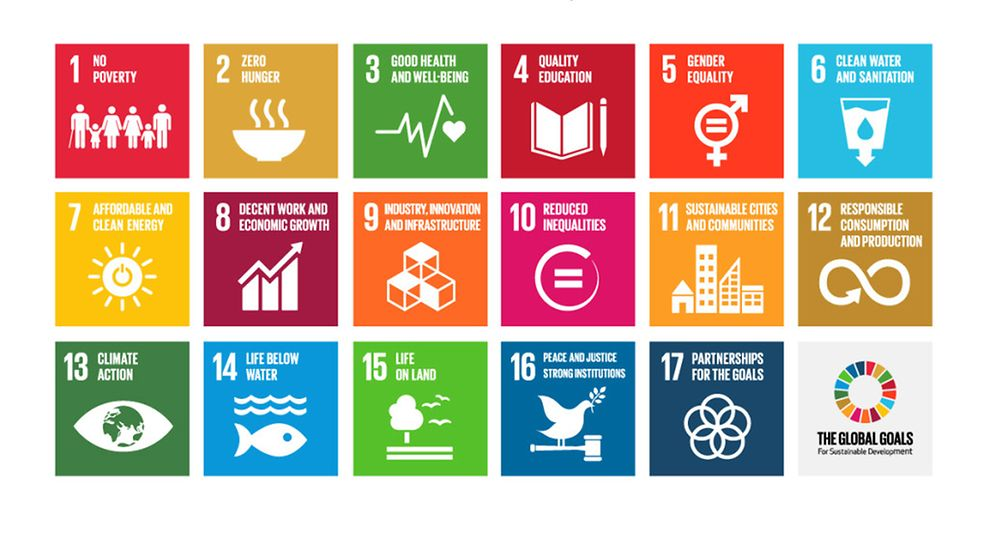
\includegraphics[width=\linewidth]{images/kacheln-the-global-goals.jpg}
	\caption{Overview of \acrfullpl{sdg} numbered from 1 to 17, adapted from The 2030 Agenda by Bundesregierung Deutschland, 2022 \cite{pic:eu_goals}.}
	\label{fig:sustainGoals}
\end{figure}


\subsection{Sustainability Targets}\label{subsec:sustainabilityGoals}
In the discussion on sustainability, the service sector is involved in almost all goals listed by the EU. The numbering of all specified goals can be seen in figure \ref{fig:sustainGoals} and are listed as follows:\\
\begin{tabular*}{\textwidth}{lclc}
	\hline
	1 & No Poverty & 9 & Industry, Innovation And Infrastructure\\
	2 & Zero Hunger & 10 & Reduced Inequalities\\
	3 & Good Health and Well-Being & 11 & Sustainable Cities \& Communities\\
	4 & Quality Education &	12 & Responsible Consumption \& Production\\
	5 & Gender Equality & 13 & Climate Action\\
	6 & Clean Water \& Sanitation & 14 & Life Below Water\\
	7 & Affordable \& Clean Energy & 15 & Life On Land\\
	8 & Decent Work \& Economic Growth & 16 & Peace \& Justice, Strong Institutions\\
	\hline
\end{tabular*}
\vskip
While providing good paying jobs through less physically intensive work, and easily accessible education, coordination services, IT and office work provides positive influences to goals regarding economic prosperity, equality and innovation (1, 2, 4, 5, 8, 9 and 10). As such the positive influences of work in this sector should be sustained as much as possible. On the other hand, service sector corporations can actively create challenges to physical and mental well being, manifested in \gls{sdg} number 3, as IT occupations are often sedentary and mentally demanding. Goals regarding Sustainable consumption, city development, institutional regulation and clean environment needs (\glspl{sdg} 6, 11, 12 and 16) can be at odds with the needs of the IT sector, due to the push to urbanization by office jobs, the variety of supply needs in modern offices. While mostly being neutral to almost all other goals, after the initial challenges are met, the sustainability can be threatened with respect to affordable and clean energy (goal 7) simply due to the existence of fully supplied offices in a developed country. Energy demands due to production, operation and demolition are a constant byproduct of economic activity in the service and IT sector. In order to facilitate the positives of office work, our goal should be to minimize negative effects in these specific other areas. Energy efficiency is an adequate tool to mitigate parts of the damages ensued due to office economy. However, to find effective ways to curb electricity consumption in all areas, a solid knowledge foundation is key, to compare and evaluate problems and solutions in the field. On the side of energy generation it is important to analyze the technical and political framework to energy availability, and the respective environmental costs.  
\begin{figure}
        \centering
        \begin{tabular}{ccc}
        	\subgraphics{GOAL_7_TARGET_7.3.png}{}&
        	\subgraphics{GOAL_9_TARGET_9.C.png}{}&
        	\subgraphics{GOAL_11_TARGET_11.6.png}{}\\
        	\subgraphics{GOAL_12_TARGET_12.6.png}{}&
        	\subgraphics{GOAL_12_TARGET_12.8.png}{}&
        	\subgraphics{GOAL_13_TARGET_13.3.png}{}
        \end{tabular}
        \caption{Collection of targets concerned by energy efficiency adapted from Global Goals, 2022 via 'https://www.globalgoals.org/resources/'.}
        \label{fig:targets}
\end{figure}  

\subsection{National Goal Implementations}\label{subsec:nationalGoals}
As a member of the European Union, the german government for the first time enacted in 2019 the respective goals into national policy with an agenda tackling every sustainability goal with the following points:\pagebreak
\begin{itemize}
	\item Human well-being and capabilities, social justice (SDGs 3, 4, 5, 8, 9, 10)
	\item Climate action and energy transition (SDGs 7, 13)
	\item Circular economy (SDGs 8, 9, 12)
	\item Sustainable building and transport (SDGs 7, 8, 9, 11, 12, 13)
	\item Sustainable agricultural and food systems (SDGs 2, 3, 8, 12, 13)
	\item A pollutant-free environment (SDGs 6, 8, 9, 14, 15)
\end{itemize}
While adapting the goals of the European Union, the specific implementation is similarly vague, in most cases. In terms of greenhouse gas emission, these goals were defined to incorporate a reduction of emissions by 65\% until 2030 compared to the level of 1990, up to a final CO$_2$ neutrality by 2045 \cite{german_goals}.
\newpage
\section{Power Consumption as a Contributor}\label{sec:powerConsumption}
From publications by the Umweltbundesamt, around 84\% of CO$_2$ equivalent emissions are produced due to emissions regarding energy and heat generation. While the total amount of CO$_2$ emissions are receding, this partition remains almost constant \cite{co2_contrib}. Therefore in order to fulfill CO$_2$ neutrality by the year 2045, more than 80\% of the problem stems from meeting any kind of energy demands. As part of the Federal Climate Change Act of 2021, the legal binding achievement of emission neutrality was finalized.
The legal goal and methodology is posted as "Climate neutrality of the federal administration is to be achieved, in particular, through
energy savings, through the efficient provision, conversion, use and storage of energy and
efficient use of renewable energy sources and the selection of the most climatefriendly modes of transport" \cite{fccl}. While setting clear milestones in a specific time frame, the legislation only sets out a very vague set of interventions. In light of achieving these goals, this work sets out to investigate possible contributions available in the context of energy consumption in office environments. The three objectives are defined as:
\begin{itemize}
	\item[1.] Generation of a robust and reliable energy consumption data set.
	\item[2.] Estimating the direct impact of consumed electricity on CO$_2$ footprint.
	\item[3.] Use well defined \acrfullpl{kpi} to identify optimization potential in energy consumption.
\end{itemize}
The section \ref{chap:relatedworks} highlights related works intersecting with these three research aspects and the office environment.

\chapter{Related Works}\label{chap:relatedworks}
As expected by the expansive number of factors contributing to sustainability, the amount of related works is also numerous. The spectrum of different research questions reflect the many facets of the broad topic of sustainability, and needs to be differentiated in the three relevant aspects, as seen in section \ref{sec:powerConsumption}. In \ref{sec:officedata} an excerpt of literature regarding available data in the context of office buildings are shown. Section \ref{sec:co2works} gives an insight into CO$_2$ footprint estimation. Finally in section \ref{sec:potential} a few papers outlining specific efficiency possibilities are shown.
\section{Data Gathering And Office Consumption}\label{sec:officedata}
The study by Kurt W. Roth et al. \cite{roth} gives a first insight on expected data in an office environment. By calculations of estimated operation hours over a year, the distribution of energy consumption across different device types were quantified and accumulated over an estimated lifetime in commercial buildings.\\
As a template in gathering and evaluation of measurement data can be seen in the work by S. Wilhelm et al. \cite{wilhelm}. The author created a labeled energy consumption data set to provide training data of private households for algorithms and machine learning in various applications. The hardware setup fits the requirements set by the experiment of this work. Parts of the software described in section \ref{subsec:software}, was built upon the basis that was graciously provided by S. Wilhelm.

\section{\texorpdfstring{CO$_2$ Estimation}{CO2 Estimation}}\label{sec:co2works}
As CO$_2$ is emitted in various stages of the office life cycle, different aspects can be examined. The work of Suzuki et al. \cite{suzuki} gives a detailed estimation of CO$_2$ impact from construction, through operation until deconstruction using industrial statistics of manufacturers and contractors.
With respect to energy consumption specifically, the work of R.Saidur \cite{saidur} establishes an estimation of the CO$_2$ footprint created by office buildings in Malaysia. The data was split into general appliances, air conditioning and lighting, to provide a very general overview of consumption in this context. 
Both works base their CO$_2$ footprint estimation upon conversion tables which relate CO$_2$ generation to their specific energy source. However this approach does not translate equally when considering power consumption. One main reason for this, is the international power grid system, which enables free trade and consumption of energy without regard where said electricity was produced. The \acrfull{emas} proposed by the European Commission determines greenhouse intensity using the \acrfull{ghg}. This protocol is structured similarly to a traditional accounting system, by separating CO$_2$ emissions into three distinct scopes as seen in table \ref{tab:scopes}. To determine CO$_2$ footprint in this manner, it would be necessary to consult the emission report of the university's respective energy provider. As these data points depend on the respective 'Scope 1' values of the provider, a proper estimation could be made referring to CO$_2$ emission data given in their \acrfull{emas} report or, if sufficient non mandatory data is given \cite{report}, data entered into the german \acrfull{prtr}. Each register only requires an annual report \cite{prtr_law}, and are unavailable in the scope of this work. In section \ref{subsec:footprint} a case for the usage of average CO$_2$ consumption will be made.

\begin{table}[h]
	\centering
	\begin{tabular}{|ll|}
		\hline
		Scope 1: & direct emission due to energy generation, transportation, processing \\
		& and fugitive emissions
		\\ \hline
		Scope 2: & indirect emissions due to consumed purchased electricity,\\
		& and associated transportation \& distribution costs
		\\ \hline
		Scope 3: & (optional) indirect emissions due to further activities \\
		& upstream in the energy generation supply line, \\
		&for example drilling and construction of electricity trade companies 
		\\ \hline
	\end{tabular}
	\caption{Scope distinction defined in the \acrfull{ghg} Corporate Standard \cite{ghg}.}
	\label{tab:scopes}
\end{table}
\section{Efficiency Potential}\label{sec:potential} 
By researching the theoretical potential of energy savings, further interesting principles can be discovered. The article by R. Launder \cite{entropy} determines that all computation produces a minimum change in entropy of a closed computational system, due to irreversible physical processes, greater or equal to $log_e 2 \times k_b \times T$. This is also known as the 'Landauer Limit' or 'Landauer Principle', and was also shown to hold in dedicated experiments, as seen by the publication of J.P.S Peterson et al. \cite{entropy-demo}. While prohibiting real 'zero energy consumption' computations, the theoretical efficiency boundaries are far from limiting the potential efficiency gains through modern interventions.\\
A field study by Victor Zhirnov et al. \cite{min-energy} gave a qualitative overview of energy consumption of different parts of computer processing, with 42\% of energy consumed by Displays, 35\% by computing, 19\% by communication and about 4\% by storage. Furthermore an increase in energy efficiency in processor computation with respect to circuit size was shown, as switching energy per transistor is decreasing. During experimentation, the specific consumption ratios can be compared to the data given here.\\
In Pereira et al. \cite{Pereira} the power consumption of 26 different programming languages was compared on a small collection of standard problems. The results show a clear superiority of compiled languages compared to interpreted languages in terms of energy efficiency. Although not in every case, the efficiency with respect to time performance correlate very closely to total power consumption. This also means that the quality of work will have great influence in expected outcomes. This could introduce unaccounted differences in consumption patterns.\\
\chapter{Physics Fundamentals}\label{chap:fundamentals}
The section \ref{sec:measurement} establishes a short overview of the physical quantities relevant to be measured by the instruments in order to determine power consumption. Section \ref{sec:vflux} introduces the considerations of noise encountered during measurement due to voltage fluctuations. 
\section{Physical quantities}\label{sec:measurement}
To establish a robust data basis, a compressed investigation on the physical fundamentals has to be made, in order to ensure a realistic expectation on the available data can be expected.
Instantaneous electrical power (P) is defined as the derivative of electrical energy over at time $t_{0}$. Electrical energy (W) is the combination of the electric current (I), defined as transported charge (Q) over time, and the electric voltage (V) of electric particles moving in an electric circuit/cite{Hacker2020}. Given the measurement of each quantity is determined as the average value over a measurement interval, all quantities are also defined as constant over the given time period. Therefore the relevant electric properties of the system can be described by the simplified formula shown in equation \ref{eq:electric formula}. 
\begin{equation}
	W = P \times t = I\times V \times t = V \times Q
	\label{eq:electric formula}
\end{equation}
By observation of the formula, the act of measuring the amount of power consumed in an electrical system is accomplished by determining the electrical potential and electrical current in a system over a given amount of time.

\section{Voltage Fluctuations}\label{sec:vflux}
The first component of interest is the voltage provided by the outlets used in IT application environments. In European countries, the amount and fluctuations of the electric grid is regulated in European standard '\gls{EN} (EN) 50160'.
By this standardization boundaries on frequency, voltage fluctuation, flickering, faults and other quantities were given. As most regulations regard the quality and safety of the power grid, an overview on relevant standards for measurement needs is given in table \ref{tab:en50160}. Due to the given voltage fluctuation ranges, a theoretical measurement error of 10\% could be expected on instantaneous measurements, due to noise in the mean voltage value of 230V.  As quality standards also demand the fluctuations to be ideally symmetrical, noise in the voltage supplied should mostly cancel out when averaging over multiple measurements.
For this reason, a method with a sufficient surplus of separate measurements, averaged over a larger time span, should be considered preferable. In this thesis, the fluctuations in measurement due to voltage issues is considered negligible.

\begin{table}[ht]
	\centering
	\begin{tabular}{|c|c|}
		\hline
		frequency & 50 Hz (+/- 1\%) \\
		\hline
		voltage fluctuation (slow) & 230 V (+/- 10\%) \\
		\hline
		voltage fluctuation (fast) & 230 V (+/- 5\%) \\
		\hline
		voltage faults (short) & < 1000 per year\\
		\hline
		voltage faults (long) & < 50 per year\\
		\hline
	\end{tabular}
	\caption{extract of standardization values given in EN 50160 \cite{EN50160}.}
	\label{tab:en50160}
\end{table}

\section{Determining Electric Current}\label{sec:current}
By analyzing the electric formula of equation \ref{eq:electric formula} and the conclusion of section \ref{sec:vflux} the power measurement is directly correlated to the electrical current an office appliance is drawing from the grid. In electrical engineering, different methods to determine the current in an electric circuit are known. The most direct way would consist of a separately closed electric circuit where voltage drops on a standardized resistor. However, this approach does not allow the observation of an already established supply system. The application of measuring 'in-use' appliances, requires different methods, like the usage linear current hall effect sensors.

\subsubsection{Hall Effect}
The hall effect is a physical phenomenon, named after US physicist Edwin Hall: 1855 – 1938. The effect "...occurs in a current-carrying conductor
that is located in a magnetic field. Thereby an electric field builds up which is perpendicular to the current direction and the magnetic field and compensates the Lorentz force affecting the electrons" \cite{Hacker2020_Hall}.
In figure \ref{fig:hall_sensor_block} a depiction of the hall sensor and its components can be viewed. Basically the conducting sheet measures a permeating magnetic field 'H' by the voltage differential '$V_H$' created through Lorentz forces (F$_L$) affecting the 'Constant Current Flow'. This is possible, as the hall voltage is rising, until its equivalent electric force (F$_e$) creates an equilibrium. The electric field strength (E) is equivalent to the hall voltage (V$_H$) divided by the diameter of the conductor plate (d)The strength the Lorentz force is directly proportional to the strength of the magnetic field (B), as well as drift velocity (v) and charge (q) of the current. The drift velocity of the particles is dictated by the current and cross section of the conductor. All relevant quantities can be computed using formula \ref{eq:hall_formula}.
\begin{equation}
	F_e = E \times q = \frac{V_H}{d} \times q =  B \times v \times q = F_L
	\label{eq:hall_formula}
\end{equation}
Rearranged the strength of the directional magnetic field is computed as shown in equation \ref{eq:hall_formula_rearranged}.
\begin{equation}
	B = \dfrac{V_H}{d \times v}
	\label{eq:hall_formula_rearranged}
\end{equation}
As every flowing current induces an electromagnetic field around the conduction it is traversing, the hall effect can be utilized to directly measure the current of a nearby electric circuit. Depending on the design of the sensor unit, the direction of electric current (positive or negative) can be distinguished. With additional amplification, trim settings and filtering, a clearer signal can be deduced, as alternating current does not produce a constant electromagnetic field. These sensors often are designated as linear current hall effect sensors. A simplified block diagram of such a hall sensor can be seen in figure \ref{fig:lcs_block}
\begin{figure}[th]
	\centering
	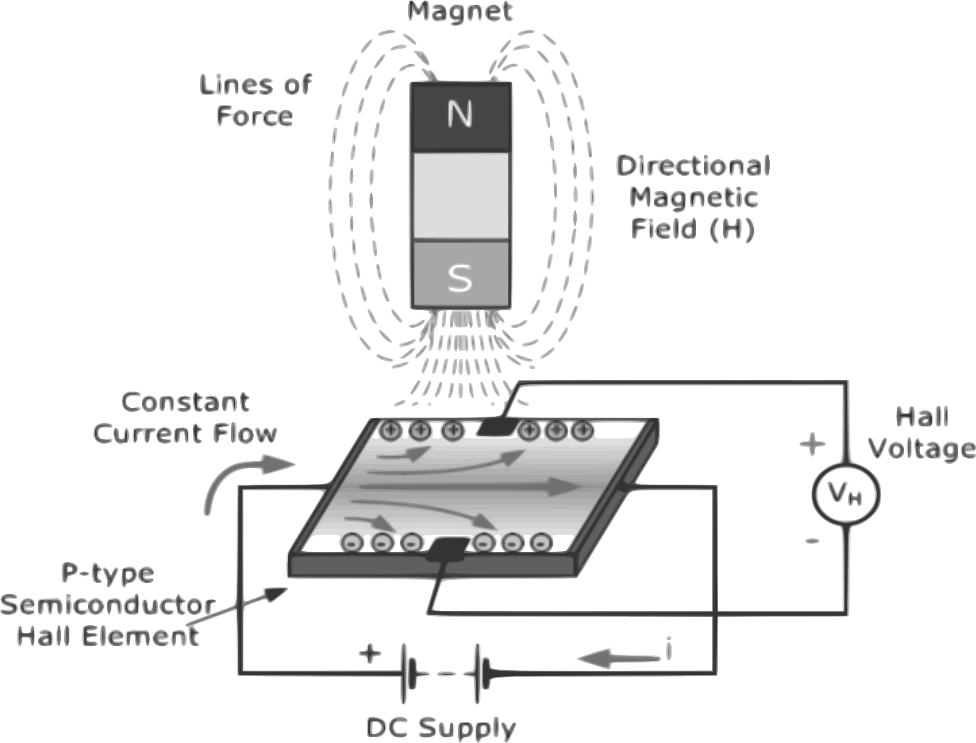
\includegraphics[width=\textwidth]{images/hall_sensor2.png}
	\caption{Block Diagram of an exemplary hall effect sensor. Recreated from \cite{hall_sensor}.} 
	\label{fig:hall_sensor_block}
\end{figure}

\begin{figure}[th]
	\centering
	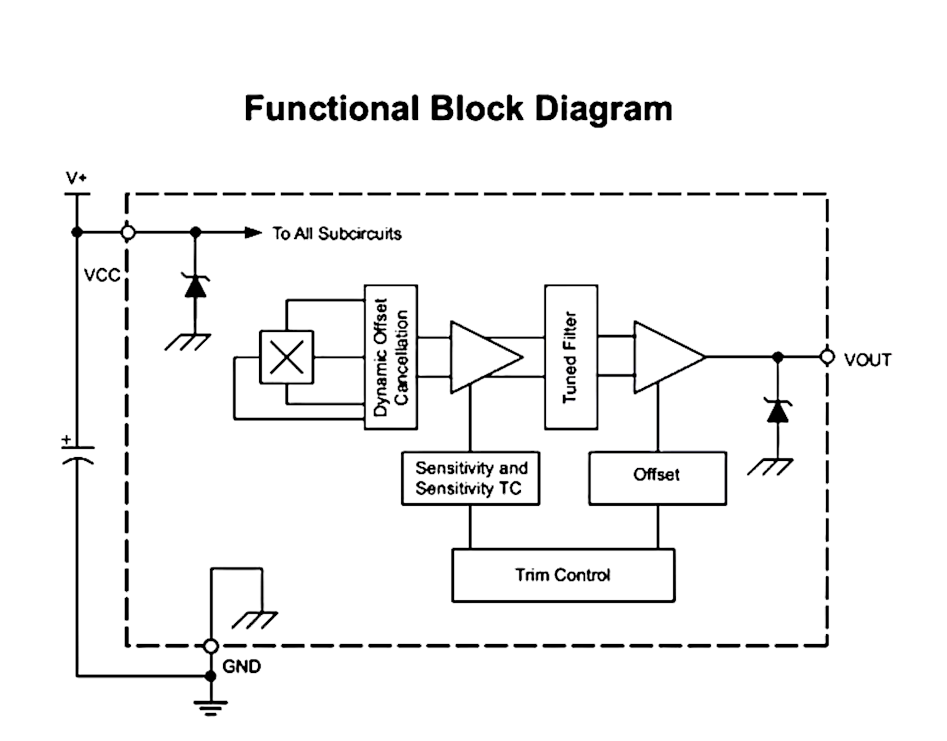
\includegraphics[width=\textwidth]{images/lcs_block_diagram.png}
	\caption{Block Diagram of an exemplary linear current hall effect sensor. The box marked with an X is signifying the hall sensor \cite{hall_effect_element14}.} 
	\label{fig:lcs_block}
\end{figure}

\section{Summary}
The conclusion of this section is, that using an assortment of hall effect sensors, the accurate measurement of flowing current in a live IT environment is very possible. As current through the electric appliance is a direct result of the energy needs of the measured object, the resulting measurement is sufficiently linked to real energy consumption.
Regarding voltage, the exact amount of the quantity is highly dependent on the power quality supplied by the grid. As this factor is mostly independent from the experiment, fluctuations and uncertainties should be reduced by using average measurements over a longer period of time. This can be achieved by evaluating the average of multiple measurements in the order of magnitude of multiple tens or hundred. For this experiment a timing window of 15 minutes is considered as sufficient, and will be chosen as the default measurement interval after averaging.

\pagebreak

\clearpage
\chapter{Methods}\label{chap:methods}

\section{Measurement Equipment}\label{sec:measurement}

\subsection{Power Consumption}\label{subsec:powerMeasurement}

\subsection{Office Attendance}\label{subsec:attendance}

\subsection{Database and Networking}\label{subsec:databaseNetworking}

\section{Evaltuation Metrics \& Tools}\label{sec:metricsTools}

\subsection{\acrfullpl{kpi}}\label{subsec:KPI}

\subsection{\acrfull{rpmt}}\label{subsec:RPMT}

\chapter{Results}\label{chap:results}

In this chapter an overview over the different evaluations and exploration tools created in this work is given. To acquire results, a short description of the processing is provided in section \ref{sec:results}. The section \ref{subsec:result_tables} shows several result tables and describes how to read and interpret the specific values.  As a few examples of evaluating the \glspl{kpi}, in section \ref{sec:visuals} a collection of visualization can be seen.
\section{Result Evaluation}\label{sec:results}
To evaluate the data set a collection of processing was done using the sql alchemy package, similar to the insert mechanism of the measurement values in the consumer paragraph of section \ref{subsec:software}. Additionally normalized tables, containing standardized 15 min intervals were created (refer to the 'Sensor\_Meta\_tables') to visualize a longer time amount in the visualization tool (refer to section \ref{subsec:RPMT}). Due to hardware and connection difficulties, data of sensor 32 did not suffice for evaluation, and has been omitted in all tables. The values of the tables in section \ref{subsec:result_tables} allow comparison of total consumption measurements, minima, maxima and averages, which were processed using SQL queries. The values are calculated similar to the equations \ref{eq:min}, \ref{eq:max} and \ref{eq:avg} respectively. 
\begin{equation}\label{eq:min}
	MIN (X) = x_i \bigg\rvert x_i, x_j \in X \wedge \not \exists x_j \geq x_i \wedge i < j
\end{equation}

\begin{equation}\label{eq:max}
	MAX (X) = x_i \bigg\rvert x_i, x_j \in X \wedge \neg \exists x_j \geq x_i \wedge i < j
\end{equation}

\begin{equation}\label{eq:avg}
	AVG (X) = \dfrac{\sum_{i=1}^{n}{x_i}}{n} \bigg\arrowvert x_i \in X \wedge |X| = n 
\end{equation}
To enable quick reference, the section \ref{subsec:insights} collects key observations gathered from the results, and shows relations that were expected by related works.
\subsection{Quantitative Results}\label{subsec:result_tables}
As a reference, the average consumption values of user 1 per day, can be seen in table \ref{tab:user1}. Date values range from 1st of June to 29th of Juli, where only weekdays are considered. The respective average values give information on the consumption rate of the specific day, while the ratio of the averages show a difference in energy conservation during off work hours. The evaluation shows two levels of days with no work activity. These days are recognizable by consumption values around 0.6 to 1.4 watts of average consumption, and virtually no difference between weekday - and workday average. The small difference between the 0.6 Watt values (e.g. 12th to 15th of Juli) and the 1.4 Watt values (e.g. 6th and 7th of June) could be explained due to for example a single device in standby (e.g. the monitor). Most activity days show good \acrshort{wwcr} values around 2, with single outliers like 21st, 22nd and 25th of Juli, that lack any consumption reduction during off hours. On the whole the average of user 1 fits the expectations of a user that is predominantly conscious of energy efficiency, while showing signs of inconsistency.\\
\begin{table}
	\centering
	\begin{tabular}{|l|c|c|}
		Date& weekday average (W)& workday average (W)\\
		2022-06-01&     7.1246&     6.3368\\
		2022-06-02&   62.9861&    86.5046\\
		2022-06-03&  66.9280 &   88.5383\\
		2022-06-06 &  1.3643 &    1.3644\\
		2022-06-07&   1.3649 &    1.3698\\
		2022-06-08&  41.0420 &   82.9115
		\\ 2022-06-09 & 23.3274 &   47.8767
		\\ 2022-06-10  & 1.3873 &    1.3913
		\\ 2022-06-13  &27.9845 &   58.8300
		\\ 2022-06-14  &25.1870 &   54.9713
		\\ 2022-06-15  &26.6638 &   42.9791
		\\ 2022-06-16  & 1.4900 &    1.4924
		\\ 2022-06-17  & 1.1917 &    1.1950
		\\ 2022-06-20  &27.2710 &   52.8197
		\\ 2022-06-21  & 0.6530 &    0.6566
		\\ 2022-06-22  &24.2942 &   46.9040
		\\ 2022-06-23   &1.1986 &    1.1995
		\\ 2022-06-24   &1.1978 &    1.1989
		\\ 2022-06-27   &1.1941 &    1.1971
		\\ 2022-06-28   &1.1968 &    1.1994
		\\ 2022-06-29   &1.1948 &    1.1964
		\\ 2022-06-30  &26.1305 &   53.3058
		\\ 2022-07-01  &1.1950   &  1.1951
		\\ 2022-07-04  &25.0155  &  50.5588
		\\ 2022-07-05   &0.6521 &    0.6518
		\\ 2022-07-06  &16.1277&    30.7782
		\\ 2022-07-07   &0.6357&     0.6368
		\\ 2022-07-08   &0.6367&    0.6365
		\\ 2022-07-11  &18.3418&  42.5024
		\\ 2022-07-12   &0.6354&    0.6352
		\\ 2022-07-13   &0.6340&     0.6345
		\\ 2022-07-14   &0.6331&     0.6321
		\\ 2022-07-15   &0.6328&     0.6344
		\\ 2022-07-18  &21.9215&    44.9616
		\\ 2022-07-19  &20.3028&    41.4121
		\\ 2022-07-20  &34.3390&    51.1681
		\\ 2022-07-21  &43.7019&    43.7787
		\\ 2022-07-22  &43.7082&    43.7739
		\\ 2022-07-25  &22.2650&    16.1565
		\\ 2022-07-26  &25.6874&    54.4252
		\\ 2022-07-27  &22.0577&    45.2281
		\\ 2022-07-28  &28.0511&    53.5048
		\\ 2022-07-29   &1.0874&     1.0907
	\end{tabular}
	\caption{Consumption results of user 1 in Watts.}
	\label{tab:user1}
\end{table}
The tables \ref{tab:sensor} and \ref{tab:sensor_cont} show the number of available measurement days, their average values and \acrfull{wwcr}. The tables give an individual insight into specific average weekday consumption, which is useful to estimate electricity demands of similar devices. As the number of days approach the 55 days duration of the evaluation range, the resulting values increase in accuracy. The addition of workday averages is then used to compute the \acrshort{wwcr} of each device respectively. This ratio can be used as an indicator to differentiate users and devices that actively reduce consumption outside of work hours. It can be clearly seen that unused sensor outlets possess a \acrshort{wwcr} of about $1$ while values from around 1.3 show little active consumption reduction during off hours. On the other extreme values around 2.3 show a great change of consumption during off hours, which either shows extremely high consumption which would be indicated by a very high \gls{workday} value, or a great reduction which is mostly indicated here.\\
The evaluation of different workplaces gain little insight as max consumption spike way higher in Mutli devices, which indicates, that workplaces are not really comparable to each other, as consumption differs greatly. Furthermore the higher amount of false 'negative' consumption in the unused working spaces further distort the consumption data elements in the data set. As almost all the \acrshortpl{wwcr} of negative sensor averages approximate 1, the odd values can be attributed to bias of the sensor, as noise should impact the averages slightly differently. The surprising value of 0.4 \acrshort{wwcr} returned on sensor 16 can be seen as a product of noise due to the low numeric values in the milliwatts range. Positive average measurements contain low frequency occupation of workplaces like sensor 28 and 29 due to low averages.\\
\begin{table}[h]
	\centering
	\begin{tabular}{l|c|c|c|c}
		Sensor Number & \# of days & weekday avg (W) & workday avg (W)& workday to weekday ratio \\
		1 & 55 & 5.3293 & 8.8202 & 1.6550 \\
		2 & 12 & 8.0936 & 13.6496 & 1.6865 \\ 
		3 & 55 & 5.8806 & 9.5379 & 1.6219  \\ 
		4 & 55 & 2.0053 & 4.0004 & 1.9948 \\
		5 & 55 & 1.9414 & 4.0445 & 2.0833 \\
		6 & 54 & 2.8747 & 5.8710 & 2.0423 \\ 
		7 & 51 & 5.8539 & 10.1643 & 1.7363  \\ 
		8 & 55 & 3.5986 & 7.9214 & 2.2012 \\
		9 & 55 & 3.6589 & 8.1175 & 2.2186 \\
		10 & 55 & 1.4391 & 3.0190 & 2.098 \\
		11 & 55 & 2.2525 & 4.6371 & 2.0586 \\ 
		12 & 55 & 0.1333 & 0.1426 & 1.0690 \\
		13 & 55 & 6.7418 & 10.2663 & 1.5228 \\
		14 & 55 & 0.3329 & 0.4553 & 1.3676 \\
		15 & 55 & 0.0672 & 0.1052 & 1.5660 \\
		16 & 55 & -0.0668 & -0.0333 & 0.4980 \\
		17 & 55 & 1.6774 & 3.5020 & 2.0877 \\
		18 & 55 & 2.2333 & 4.6420 & 2.0786 \\
		19 & 55 & -0.1789 & -0.1780 & 0.9948 \\
		20 & 55 & -0.0805 & -0.0804 & 0.9990 \\ 
		21 & 55 & -0.0880 & -0.0878 & 0.9987 \\
		22 & 55 & 17.3964 & 18.2880 & 1.0512 \\
		23 & 55 & 6.8836 & 14.1276 & 2.0523 \\
		24 & 55 & 2.3189 & 4.8253 & 2.0809 \\
	\end{tabular}
	\caption{Result table of average \gls{workday}, and weekday consumption of sensor 1 to 24 in Watts. Continuation follows in table \ref{tab:sensor_cont}.}
	\label{tab:sensor}
\end{table}
\begin{table}[h]
	\centering
	\begin{tabular}{l|c|c|c|c}
		Sensor Number & \# of days & weekday avg & workday avg & workday to weekday ratio \\
		25 & 55 & 3.5589 & 7.4198 & 2.0848 \\
		26 & 55 & 3.4856 & 6.9230 & 1.9862 \\
		27 & 55 & 0.1361 & 0.1875 & 1.3776 \\
		28 & 55 & 0.5605 & 1.2871 & 2.2964 \\
		29 & 55 & 2.2456 & 4.4983 & 2.0032 \\
		30 & 55 & 17.6872 & 27.9409 & 1.5797 \\
		31 & 55 & -0.1473 & -0.1462 & 0.9922 \\
		33 & 55 & 10.4353 & 20.2452 & 1.9401 \\
		34 & 55 & 4.7989 & 8.5369 & 1.7789 \\
		35 & 55 & 0.7072 & 0.8253 & 1.1670 \\
		36 & 55 & 27.0940 & 36.2963 & 1.3396 \\
		37 & 55 & 45.8122 & 65.0602 & 1.4201 \\
	\end{tabular}
	\caption{Result table of average \gls{workday}, and weekday consumption of sensor 25 to 37 in Watts. Precursory available in result table \ref{tab:sensor}.}
	\label{tab:sensor_cont}
\end{table}
To examine differences in workplace organization, tables \ref{tab:multi_wp}, \ref{tab:dual_workplace} and \ref{tab:singleworkplace} show overview values of the respective workplace type. Each table shows the corresponding Devices, their overall minimum and maximum consumption value on record, as well as the average consumption across the evaluation period. Each final row shows a 'Total' value that represents the total minimum, maximum and average of the values of the table above. This final row in each table shows the peak consumption value in them, and the respective device can be determined, and the average total consumption can again be used to estimate consumption of similar workplaces. Dual workplace evaluations contain a large number of vacant or changing occupation during the measurement period. Due to this a relevant comparison between the workplaces gives little insight in their comparison. As indicated by the maximum values, the resulting consumption should be expected to be comparable, a final evaluation does not provide this kind of conclusion. As total values of dual workplaces should be in similar ranges, the fact that averages differ beyond factor 2 cannot be easily ignored. This leads to the theory that workload and/or occupation frequency is very different between the workplaces, and the individual consumption of the users do not scale linearly in dual workplaces irrespective of the type of work and work frequency (like part time to full time employment or home office times).\\The workplace evaluation, completed by the results in table \ref{tab:singleworkplace} gives little insights when comparing absolute values. The issue is, that due to no information on the comparability of each workload in a given workplace, the reduction or increase in consumption can be explained from energy efficiency, to time efficiency with high work consumption, to normal time efficiency averaging a low work consumption.
\begin{table}[h]
	\centering
		\begin{tabular}{l|c|c|c|c}
		\multicolumn{5}{c}{Workplace 3} \\
		Device ID & Device Type & min power (W)& max power (W)& avg consumption (W)\\
		14 & PC & -0.3 & 276.4 & 2.0851 \\
		15 & Monitor & -0.3 & 15.2 & 0.7428 \\
		16 & PC & -0.2 & 42.7 & -0.0822 \\
		17 & Monitor & -0.4 & 13.2 & 0.8994 \\
		18 & Monitor & -0.3 & 17.5 & 1.1453 \\
		19 & PC & -0.3 & 15.8 & -0.1230 \\
		20 & Monitor & -0.2 & 44.6 & -0.0705 \\
		21 & Monitor & -0.2 & 0.0 & -0.0885 \\
		22 & Printer & -0.2 & 2671.0 & 16.4998 \\
		\hline
		Total & Multiple & -0.4 & 2671.0 & 21.0078
	\end{tabular}
	\begin{tabular}{l|c|c|c|c}
		\multicolumn{5}{c}{Workplace 4} \\
		Device ID & Device Type & min power (W)& max power (W)& avg consumption (W)\\
		23 & PC &-0.1 & 89.8 & 2.7413 \\
		24 & Monitor & -0.3 & 15.3 & 0.8937 \\
		25 & Monitor & -0.4 & 21.3 & 1.3511 \\
		26 & PC & -0.8 & 208.7 & 3.6216 \\
		27 & Monitor & -0.2 & 26.7 & 0.9517 \\
		28 & Monitor & -0.3 & 22.3 & 0.9721 \\
		29 & Monitor & -0.3 & 22.3 & 1.6204 \\
		30 & PC & -2.8 & 2152.8 & 10.2244 \\
		31 & Monitor & -0.3 & 0.0 & -0.1449 \\
		\hline
		Total & Multiple & -2.8 & 2152.8 & 22.2318
	\end{tabular} 
	\begin{tabular}{l|c|c|c|c}
		\multicolumn{5}{c}{Workplace 5} \\
		ID & Type & min power (W)& max power (W)& avg consumption (W)\\
		33 & PC & 0.3 & 243.2 & 8.2019 \\
		\hline
		Total& Multiple & 0.3 & 243.2 & 8.2019 \\
	\end{tabular}
	\caption{Result table of Workplaces of type multiple (more than 2 potential users).}
	\label{tab:multi_wp}
\end{table}
\begin{table}[h]
	\centering
	\begin{tabular}{l|c|c|c|c}
		\multicolumn{5}{c}{Workplace 1} \\
		ID & Type & min power (W)& max power (W)& avg consumption (W)\\
		4 & PC & -0.2 & 20.6 & 1.0352 \\
		5 & Monitor & -0.2 & 21.1 & 0.7207 \\
		6 & Monitor & -0.2 & 70.2 & 1.7565 \\
		7 & PC & -0.3 & 114.7 & 6.2446 \\
		8 & Monitor & -0.3 & 35.9 & 4.1898 \\
		9 & Monitor & -0.2 & 33.4 & 3.5638 \\
		\hline
		Total & Multiple & -0.3 & 114.7 o& 17.5104
	\end{tabular}
	\begin{tabular}{l|c|c|c|c}
		\multicolumn{5}{c}{Workplace 6} \\
		ID & Type & min power (W)& max power (W)& avg consumption (W)\\
		34 & Multiple & -0.3 & 127.9 & 6.1979 \\
		35 & Multiple & -0.4 & 105.8 & 0.5758 \\
		\hline
		Total & Multiple & -0.4 & 127.9 & 6.7738
	\end{tabular}
	\begin{tabular}{l|c|c|c|c}
		\multicolumn{5}{c}{Workplace 7} \\
		ID & Type & min power (W)& max power (W)& avg consumption (W)\\
		36 & Multiple & 10.3 & 1180.5 & 27.7893 \\
		37 & Multiple & 0.7 & 257.4 & 43.2404 \\
		\hline
		Total & Multiple & 0.7 & 1180.5 & 72.0296
	\end{tabular}
	\caption{Result table of workplaces of type Dual (exactly 2 potential users).}
	\label{tab:dual_workplace}
\end{table}
\begin{table}[h]
	\begin{tabular}{l|c|c|c|c}
		\multicolumn{5}{c}{Workplace 0} \\
		ID & Type & min power (W)& max power (W)& avg consumption (W)\\
		1 & PC & -0.2 & 91.2 & 5.8942 \\
		2 & Monitor & -0.2 & 33.3 & 5.1298 \\
		3 & Monitor & -0.1 & 33.5 & 6.6894 \\
		\hline
		Total & Multiple & -0.2 & 91.2 & 17.7135
	\end{tabular}
	\begin{tabular}{l|c|c|c|c}
		\multicolumn{5}{c}{Workplace 2} \\
		ID & Type & min power (W)& max power (W)& avg consumption (W)\\
		10 & PC & -0.2 & 18.4 & 1.1847 \\
		11 & Monitor & -0.2 & 83.4 & 1.6731 \\
		12 & Printer & -0.6 & 289.8 & 0.1327 \\
		13 & Utility & -0.2 & 2523.0 & 4.8885 \\
		\hline 
		Total & Multiple & -0.6 & 2523.0 & 7,8792
	\end{tabular}
	\caption{Result table of workplaces of type single (exactly one potential user).}
	\label{tab:singleworkplace}
\end{table}
In tables \ref{tab:PCMon} and \ref{tab:devices} a direct comparison of the individual types of devices can be made. Each table consists of the collection of devices of matching type, showing all time minimum, maximum and average consumption measurements. The respective total row of each tabular can be used to determine the consumption ratio of each type of device to the total consumption. In this instance, the multiple type broadly consist of a mixture of all other device types and is ignored in the type differentiation. Interestingly the sum of all recorded single devices almost exactly equals the total consumption of all Multi device sensors (sum of 86.34 to Multi measurement 86.01). The resulting mix of consumption computes to 38\% PC, 37\% Monitors, 6\% Utilities and 19\% through Printing. The average measured consumption adds up to 172.35 Watts and an hourly CO$_2$ footprint of 61.3 g of direct emission through electricity consumption. This gives a yearly footprint estimation of at least 0.38 tons of CO$_2$ using 260 working days a year and assuming zero emissions on the remaining days. By estimations of atmosfair, this equates to about a quarter of the estimated allowed CO$_2$ budget of a person until 2050, to remain in alignment with the Paris agreement \cite{co2_capita}. 
\begin{table}[h]
	\centering
	\begin{tabular}{l|c|c|c}
		\multicolumn{4}{c}{Device type PC} \\
		ID & min power (W)& max power (W)& avg consumption (W)\\
		1 & -0.2 & 91.2 & 5.8942\\
		4 & -0.2 & 20.6 & 1.0352 \\
		7 & -0.3 & 114.7 & 6.2446 \\
		10 & -0.2 & 18.4 & 1.1847 \\
		14 & -0.3 & 276.4 & 2.0851 \\
		16 & -0.2 & 42.7 & -0.0822 \\
		19 & -0.3 & 15.8 & -0.1230 \\
		23 & -0.1 & 89.8 & 2.7412 \\
		26 & -0.8 & 208.7 & 3.6216 \\
		30 & -2.8 & 2152.8 & 10.2244 \\
		\hline
		Total & -2.8 & 2152.8 & 32.8260 \\
	\end{tabular}
	
	\begin{tabular}{l|c|c|c}
		\multicolumn{4}{c}{Device type Monitor} \\
		ID & min power (W)& max power (W)& avg consumption (W)\\
		2 & -0.2 & 33.3 & 5.1298 \\
		3 & -0.1 & 33.5 & 6.6894 \\
		5 & -0.2 & 21.1 & 0.7207 \\
		6 & -0.2 & 70.2 & 1.7565 \\
		8 & -0.3 & 35.9 & 4.1898 \\
		9 & -0.2 & 33.4 & 3.5638 \\
		11 & -0.2 & 83.4 & 1.6731 \\
		15 & -0.3 & 15.2 & 0.7428 \\
		17 & -0.4 & 13.2 & 0.8993 \\
		18 & -0.3 & 17.5 & 1.1453 \\
		20 & -0.2 & 44.6 & -0.0705 \\
		21 & -0.2 & 0.0 & -0.0885 \\
		24 & -0.3 & 15.3 & 0.8937 \\
		25 & -0.4 & 21.3 & 1.3511 \\
		27 & -0.2 & 26.7 & 0.9517 \\
		28 & -0.3 & 22.3 & 0.9721 \\
		29 & -0.3 & 22.3 & 1.6204 \\
		31 & -0.3 & 0.0 & -0.1449 \\
		\hline
		Total & -0.4 & 83.4 &31.995 \\
	\end{tabular}
	\caption{Result table showing average consumption of PC and Monitor devices.}
	\label{tab:PCMon}
\end{table}
\begin{table}[h]
	\centering
	\begin{tabular}{l|c|c|c}
		\multicolumn{4}{c}{Device type Utility} \\
		ID & min power (W)& max power (W)& avg consumption (W)\\
		13 & -0.2 & 2523 & 4.8885 \\
	\end{tabular}
	\begin{tabular}{l|c|c|c}
		\multicolumn{4}{c}{Device type Printer} \\
		ID & min power (W)& max power (W)& avg consumption (W)\\
		12 & -0.6 & 289.8 & 0.1327 \\
		22 & -0.2 & 2671.0 & 16.4998 \\
		\hline
		Total & -0.6 & 2671.0 & 16.6324
	\end{tabular}
	\begin{tabular}{l|c|c|c}
		\multicolumn{4}{c}{Device type Multiple} \\
		ID & min power (W)& max power (W)& avg consumption (W)\\
		34 & -0.3 & 127.9 & 6.1979 \\
		37 & 0.7 & 257.4 & 43.2403 \\
		36 & 10.3 & 1180.5 & 27.7893 \\
		33 & 0.3 & 243.2 & 8.2019 \\
		35 & -0.4 & 105.8 & 0.5758 \\
		\hline
		Total & -0.4 & 1180.5 &86.0055 \\ 
	\end{tabular}
	\caption{Result table showing average consumption of Utility, Printer and Multi devices.}
	\label{tab:devices}
\end{table}

\paragraph{Idle Time} as defined in equation \ref{eq:idle} was calculated using the meta\_tables of each device, wherever available. The results can be seen in tabular \ref{tab:idle} consisting of the device, the corresponding workplace, and the resulting idle time in absolute and relative terms. While working as intended with Computer and Monitoring devices, which indicate reasonable working hours of the devices of averaging to about 4 hours of usage per workday. This should be a reasonable estimate considering 7 hour workdays dispersed with home office and holiday vacancies. Devices with higher off hour consumption like the type of printer used monitored by sensor 22 show no idle time at all, which would indicate usage without interruption. This observation does not hold when comparing consumption profiles using heat maps, as seen in section \ref{sec:visuals}.
\begin{table}[ht]
	\centering
	\begin{tabular}{|l|c|c|c|c|c|}%
		\hline%
		Sensor&Device&Workplace&Workplace Type&Idle Time&Idle Time in \%\\%
		\hline%
		Sensor 1&PC&0&Single&4909&84 \%\\%
		\hline%
		Sensor 2&Monitor&0&Single&3786&83 \%\\%
		\hline%
		Sensor 3&Monitor&0&Single&4919&84 \%\\%
		\hline%
		Sensor 4&PC&1&Dual&5023&87 \%\\%
		\hline%
		Sensor 5&Monitor&1&Dual&5116&87 \%\\%
		\hline%
		Sensor 6&Monitor&1&Dual&4546&84 \%\\%
		\hline%
		Sensor 7&PC&1&Dual&0&0 \%\\%
		\hline%
		Sensor 8&Monitor&1&Dual&4974&85 \%\\%
		\hline%
		Sensor 9&Monitor&1&Dual&4992&85 \%\\%
		\hline%
		Sensor 10&PC&2&Single&5412&92 \%\\%
		\hline%
		Sensor 11&Monitor&2&Single&5405&92 \%\\%
		\hline%
		Sensor 12&Printer&2&Single&5845&100 \%\\%
		\hline%
		Sensor 13&Utility&2&Single&0&0 \%\\%
		\hline%
		Sensor 14&PC&3&Single&5612&96 \%\\%
		\hline%
		Sensor 15&Monitor&3&Single&5706&97 \%\\%
		\hline%
		Sensor 16&PC&3&Single&5842&100 \%\\%
		\hline%
		Sensor 17&Monitor&3&Single&4908&84 \%\\%
		\hline%
		Sensor 18&Monitor&3&Single&4904&84 \%\\%
		\hline%
		Sensor 19&PC&3&Single&5856&100 \%\\%
		\hline%
		Sensor 20&Monitor&3&Single&5843&100 \%\\%
		\hline%
		Sensor 21&Monitor&3&Single&5856&100 \%\\%
		\hline%
		Sensor 22&Printer&3&Single&0&00 \%\\%
		\hline%
		Sensor 23&PC&4&Multi&4990&85 \%\\%
		\hline%
		Sensor 24&Monitor&4&Multi&5094&87 \%\\%
		\hline%
		Sensor 25&Monitor&4&Multi&5094&87 \%\\%
		\hline%
		Sensor 26&PC&4&Multi&5059&86 \%\\%
		\hline%
		Sensor 27&Monitor&4&Multi&5848&100 \%\\%
		\hline%
		Sensor 28&Monitor&4&Multi&5826&99 \%\\%
		\hline%
		Sensor 29&Monitor&4&Multi&5039&86 \%\\%
		\hline%
		Sensor 30&PC&4&Multi&5019&86 \%\\%
		\hline%
		Sensor 31&Monitor&4&Multi&5856&100 \%\\%
		\hline%
		Sensor 33&Multiple&5&Multi&0&0 \%\\%
		\hline%
		Sensor 34&Multiple&6&Dual&4309&74 \%\\%
		\hline%
		Sensor 35&Multiple&6&Dual&5762& 98 \%\\%
		\hline%
		Sensor 36&Multiple&7&Dual&0&0 \%\\%
		\hline%
		Sensor 37&Multiple&7&Dual&0&0 \%\\%
		\hline%
	\end{tabular}
	\caption{Overview of the calculated idle times of each device. The Idle Time column shows the number of intervals (15 minutes) with a power reading of less than 1 Watt.}
	\label{tab:idle}
\end{table} 

\subsection{Key Insights}\label{subsec:insights}
\noindent The device type evaluation gives parts of the expected results from the literature\cite{min-energy}, that consumption due to monitoring is very comparable to processing consumption as seen in the average consumption values of table \ref{tab:PCMon}. Apparently the different advances in energy efficiency in screens and computer performance seem to balance nicely, as literature values are more than 10 years obsolete. The difference of a few percentage points in consumption (38\% to 44\% for Monitoring, 37\% to 39\%) do not indicate huge progression differences. From another perspective, IT workers should be sensitized to the fact that dual monitor setups increase consumption by roughly 33\% compared to single monitor setups.\\
Evaluations in workplace contexts show no clear relations regarding energy consumption. Real work frequency(full time, part time or remote work), and classification of work for each user are likely the major contributor to determine total energy consumption than the individual workplace structure. This evaluation can change if the usage profile of the experiment is not representative of a usual working environment.\\
\acrfull{wwcr} delivers a suitable measure to differentiate users of similar consumption averages. This can be used to determine possible saving methodologies to increase the ratio by consumption reduction during off work hours on individuals that could harbor a greater saving potential.\\
Idle time is unsuitable for device agnostic measurements, and needs to be modified according to the expected usage profile of a specific device and the bias / noise effects on the used sensors.

\section{Visualizations}\label{sec:visuals}
Time series data is in many ways well suited to visualized. However,
to accommodate for differences in timestamp usage, all database tables created for visualization should use epoch time in milliseconds. This format is used in the sensor\_meta tables, to ease their usage in Grafana. However, different tools can require another format to visualize the time series, and the conversions can be made accordingly using simple division constants. While different applications define epoch base up to the nanoseconds, this kind of application does not benefit from higher frequencies, as HTTP requests provide a lower temporal resolution. 

\subsubsection{Heat maps}
To visualize an overview of consumption over time, in this section a collection of comparable plots are displayed. In figure \ref{fig:user_comparison} the accumulated data for each distinct user can be seen in a row, with whole day values on the left, and data limited to \gls{workday} hours on the right. A great difference in coloring between the left and right sides indicate a high \gls{wwcr} for this user. If devices between users are comparable this indicates either a high consumption during work hours or an effort of energy saving after and before work hours. This evaluation shows to be less effective with short consumption peaks, like in barely used workplaces (see fig \ref{fig:user_comparison} row 5 and 12 for reference).
As expected, differences between users regarding their \gls{wwcr} can be seen, as well as the less frequented working spaces due to their color extremes. User 14 shows little difference between \gls{workday} and weekday values, which indicates little change of energy consumption during off hours, which means a greater potential of energy efficiency gain should be expected by reducing off hour consumption. As a counter example user 10 can be examined, which shows a bigger color change and narrower distribution. Generally a drop in consumption on Fridays can be examined.  With this kind of analysis, a more directed package of intervention mechanism can be explored, to improve performance of less dedicated users with higher reduction potential. The Indication of the quantitative analysis of user 1 given in the section \ref{subsec:result_tables} using table \ref{tab:user1} can be confirmed using the heat map, as color changes can be clearly seen in comparison of the depictions in the first row. Further of interest is the visualization of user 7 which shows high consumption on weekends. This is the result of constant negative measurements due to noise and a slight sensor bias, as weekend values were not considered, which results in a 0 value in visualization. This fact especially has to be considered when handling measurements including real "negative" measurements due to localized power generation.\\
Figure \ref{fig:office_consumption} shows the summation of all power consumption on weekdays. Additionally the heat maps were generated using only specific device types. The different kinds of devices that were considered are PCs (see figure \ref{fig:pc_hm}), Monitors (see figure \ref{fig:mon_hm}), Printer (see figure \ref{fig:printer_hm}) and Utilities (see figure \ref{fig:util_hm}). As expected, the color scheme of PC consumption coincides very well with monitor usage, but not very well with printer usage. This indicates external factors to the printer usage besides attendance for example (i.e. exams or meetings/out of office gatherings). These kinds of illustrations can be useful to determine patterns in cooperation, that quantitative information does not allow. \hskip
\begin{figure}[ht]
    \centering
    \subfloat{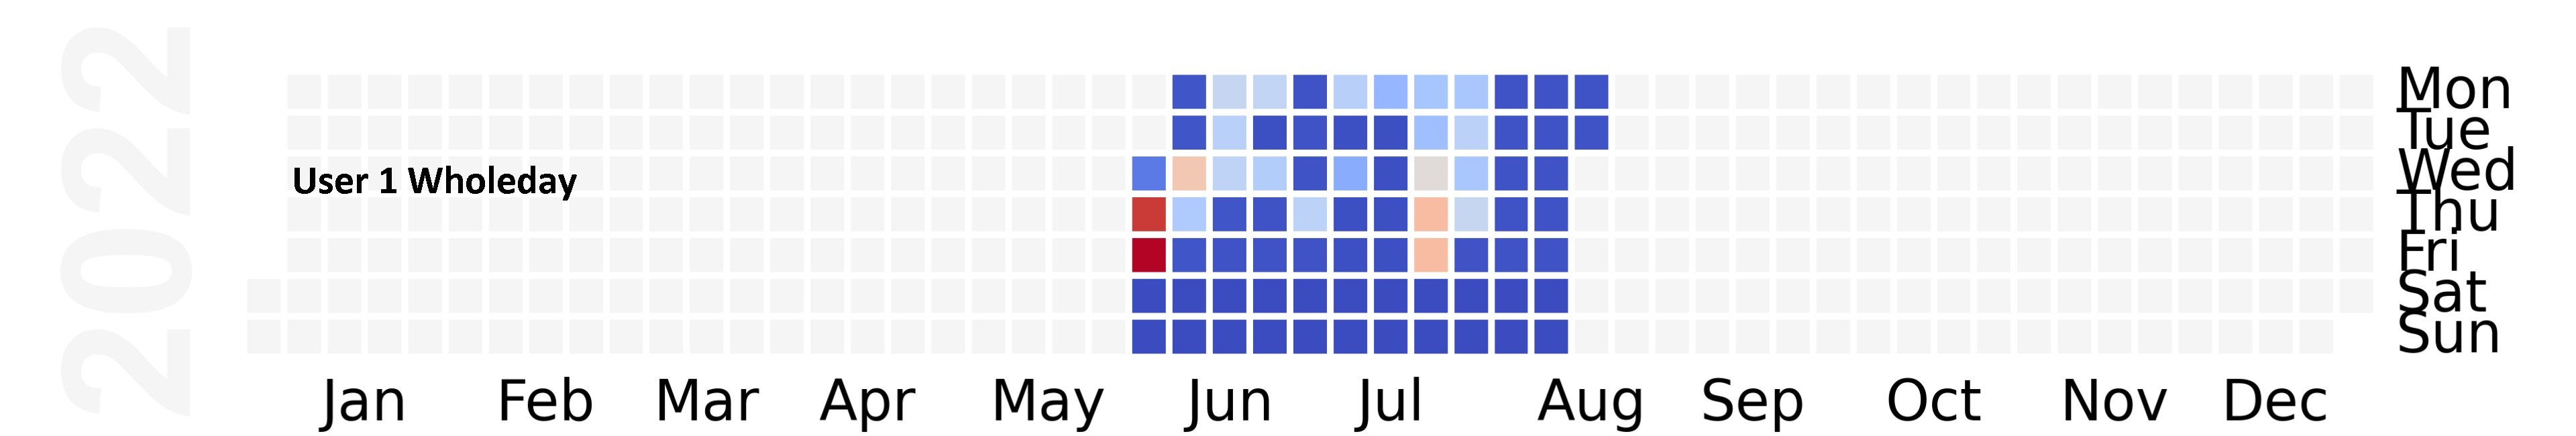
\includegraphics[width=0.5\textwidth]{images/heatmaps/user_1_wholeday_cal.png}}
    \subfloat{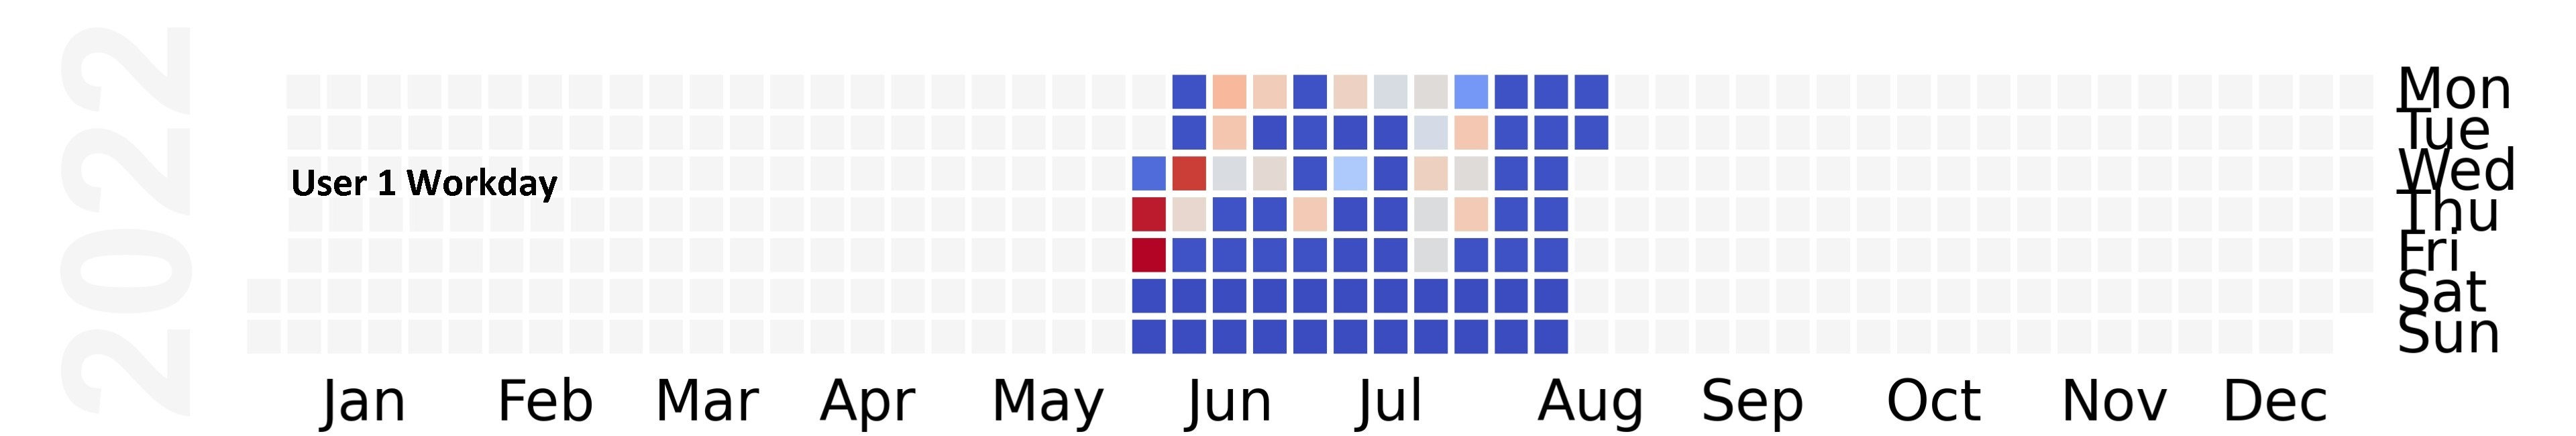
\includegraphics[width=0.5\textwidth]{images/heatmaps/user_1_workday_cal.png}}\newline
    \subfloat{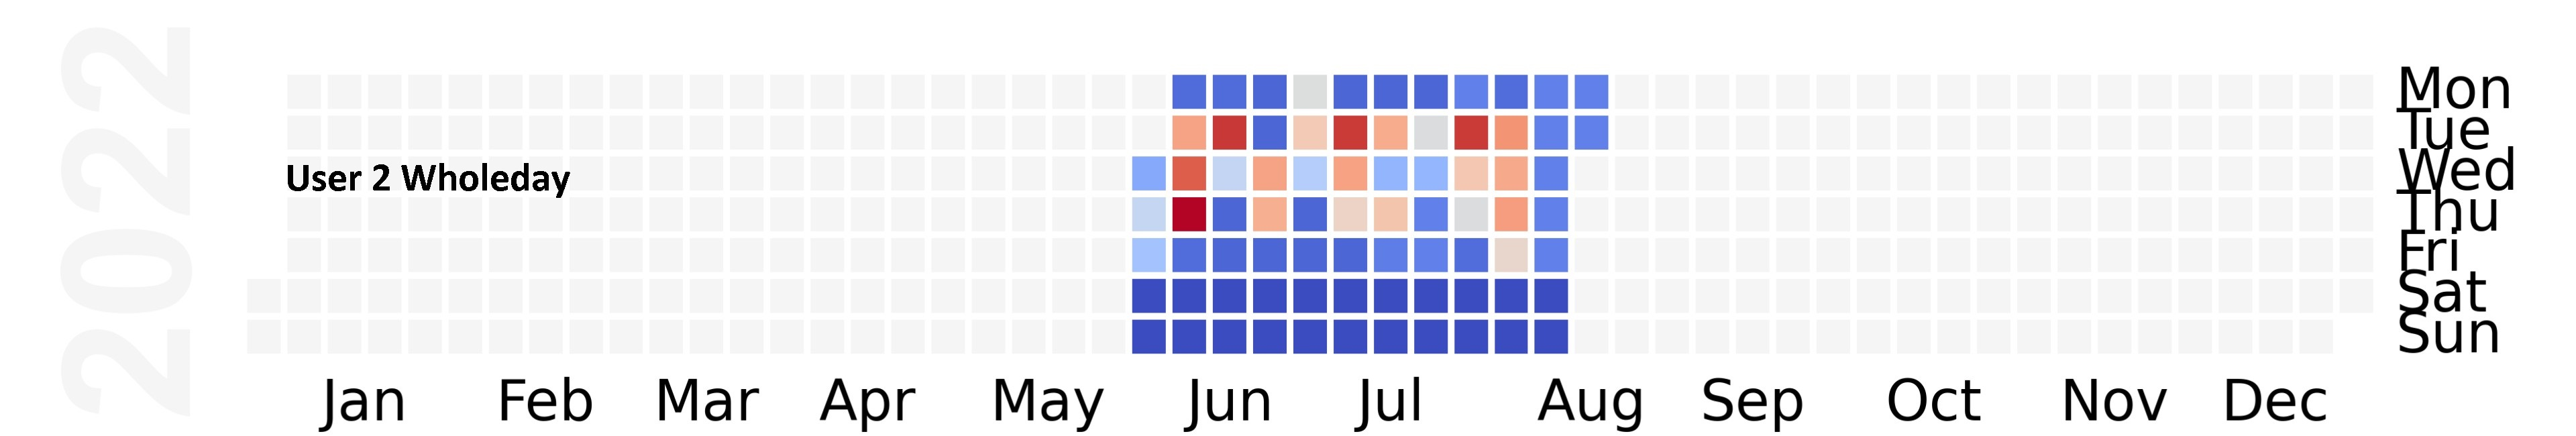
\includegraphics[width=0.5\textwidth]{images/heatmaps/user_2_wholeday_cal.png}}
    \subfloat{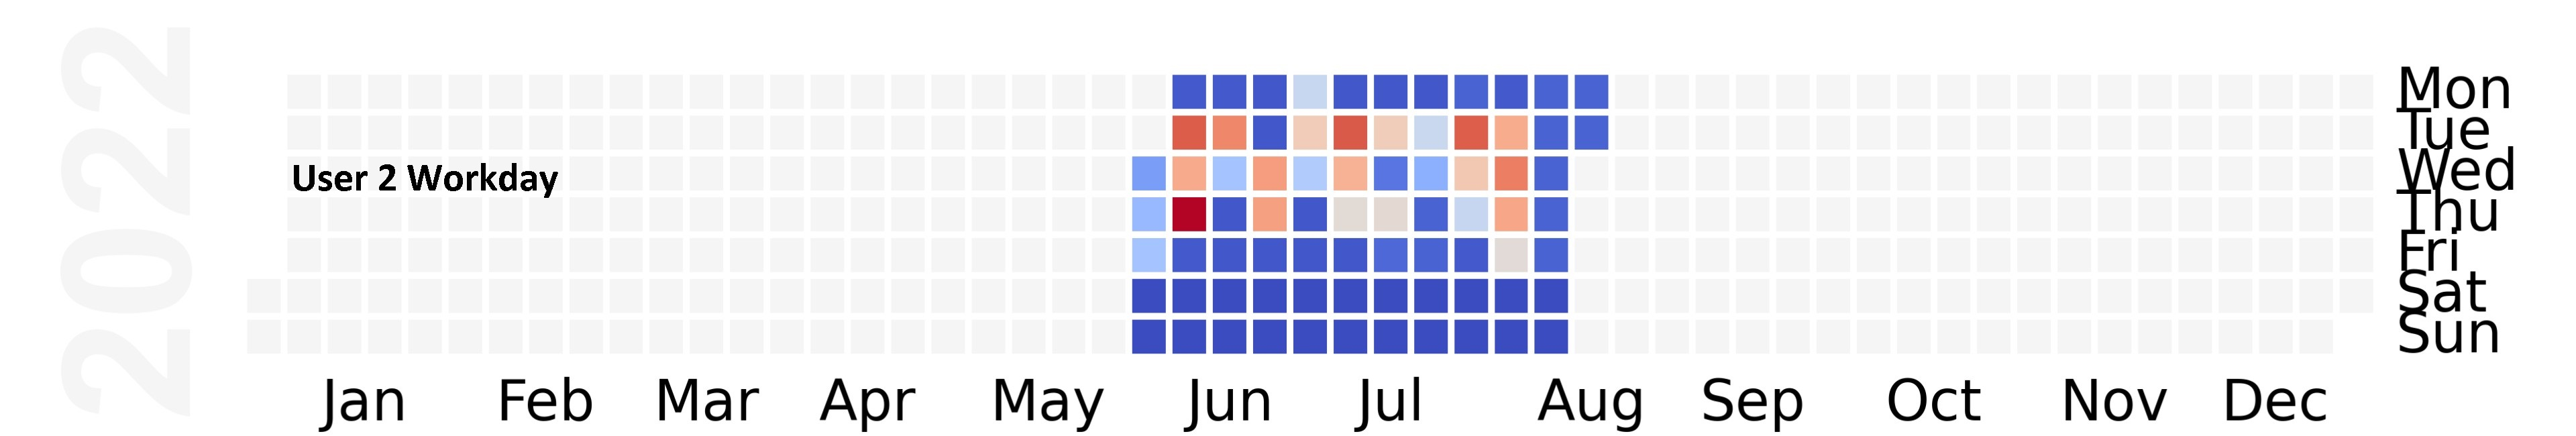
\includegraphics[width=0.5\textwidth]{images/heatmaps/user_2_workday_cal.png}}\newline
    \subfloat{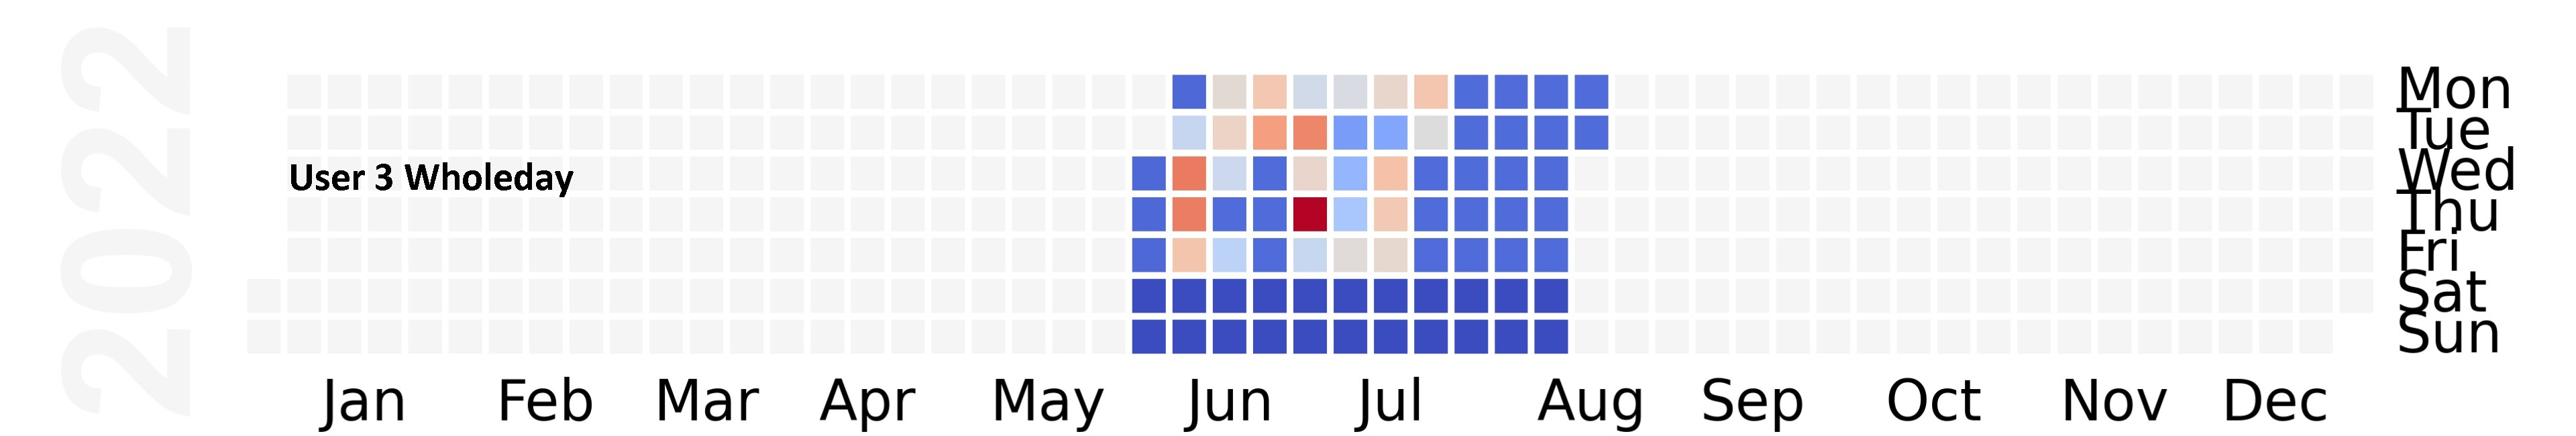
\includegraphics[width=0.5\textwidth]{images/heatmaps/user_3_wholeday_cal.png}}
    \subfloat{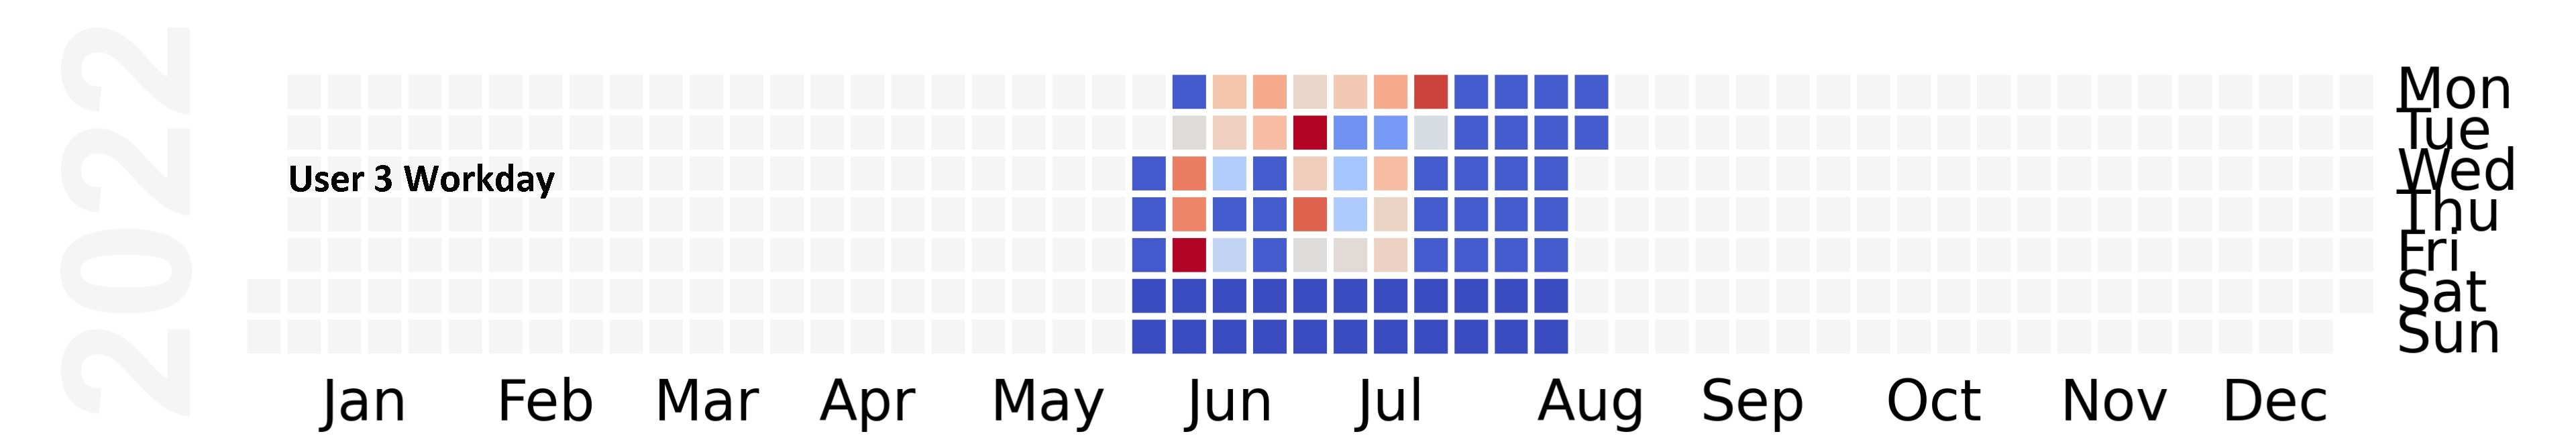
\includegraphics[width=0.5\textwidth]{images/heatmaps/user_3_workday_cal.png}}\newline
    \subfloat{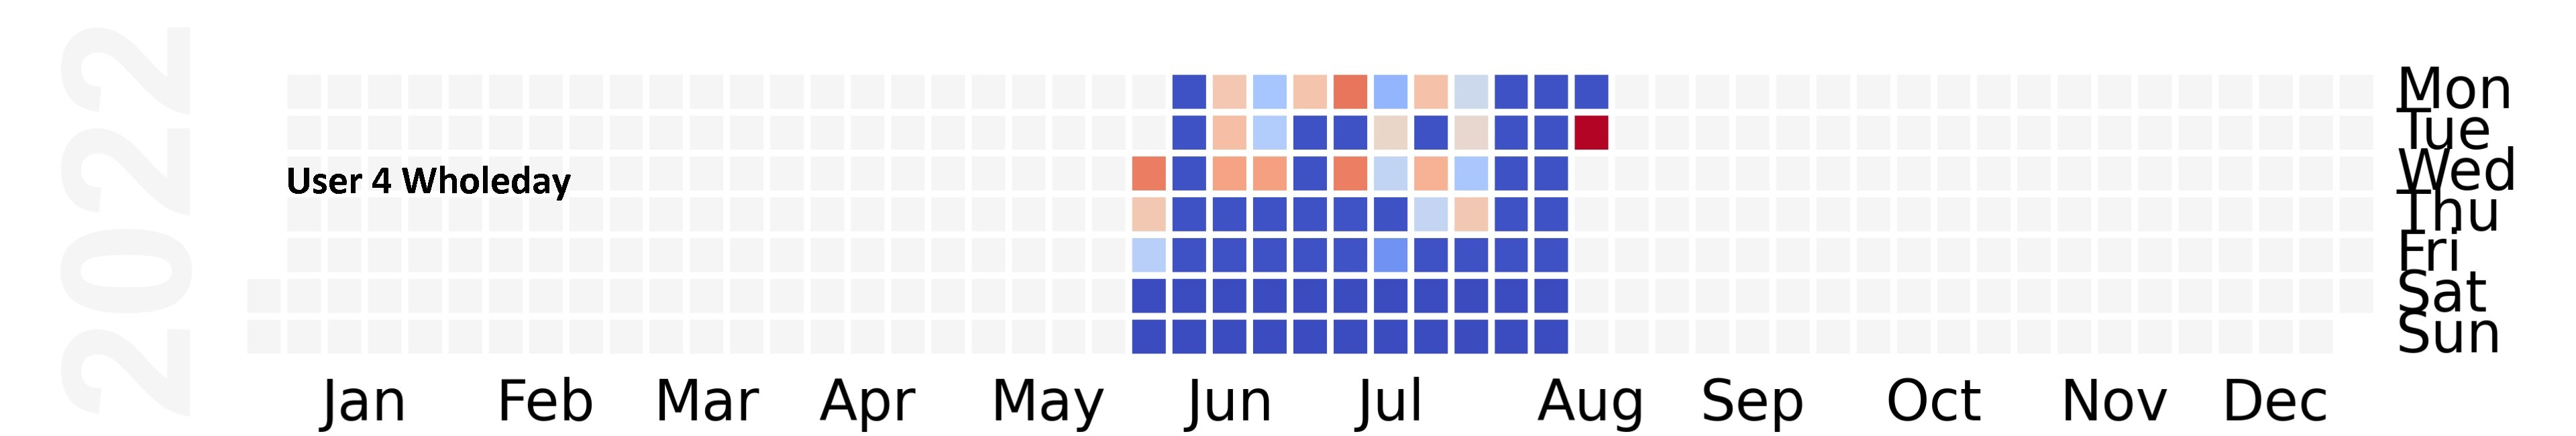
\includegraphics[width=0.5\textwidth]{images/heatmaps/user_4_wholeday_cal.png}}
    \subfloat{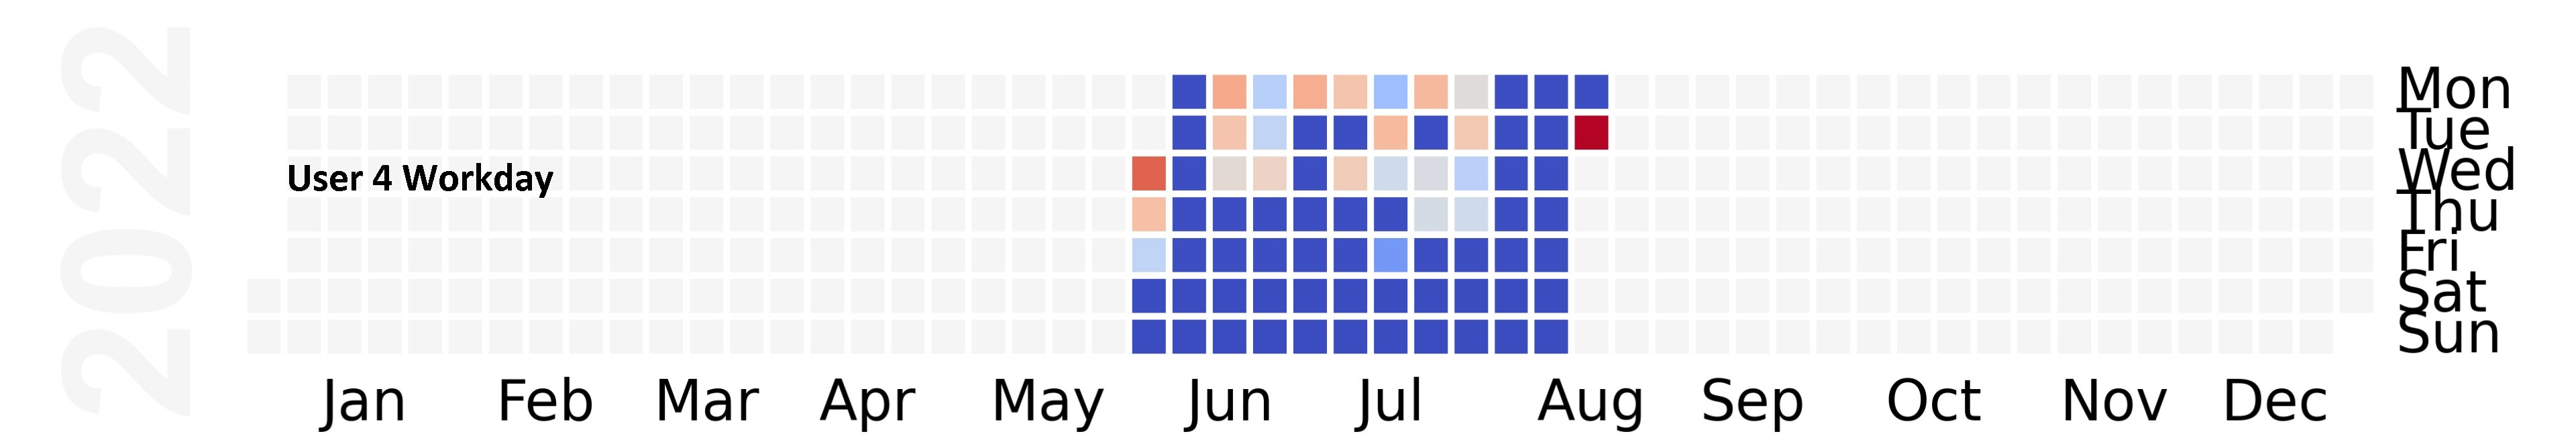
\includegraphics[width=0.5\textwidth]{images/heatmaps/user_4_workday_cal.png}}\newline
    \subfloat{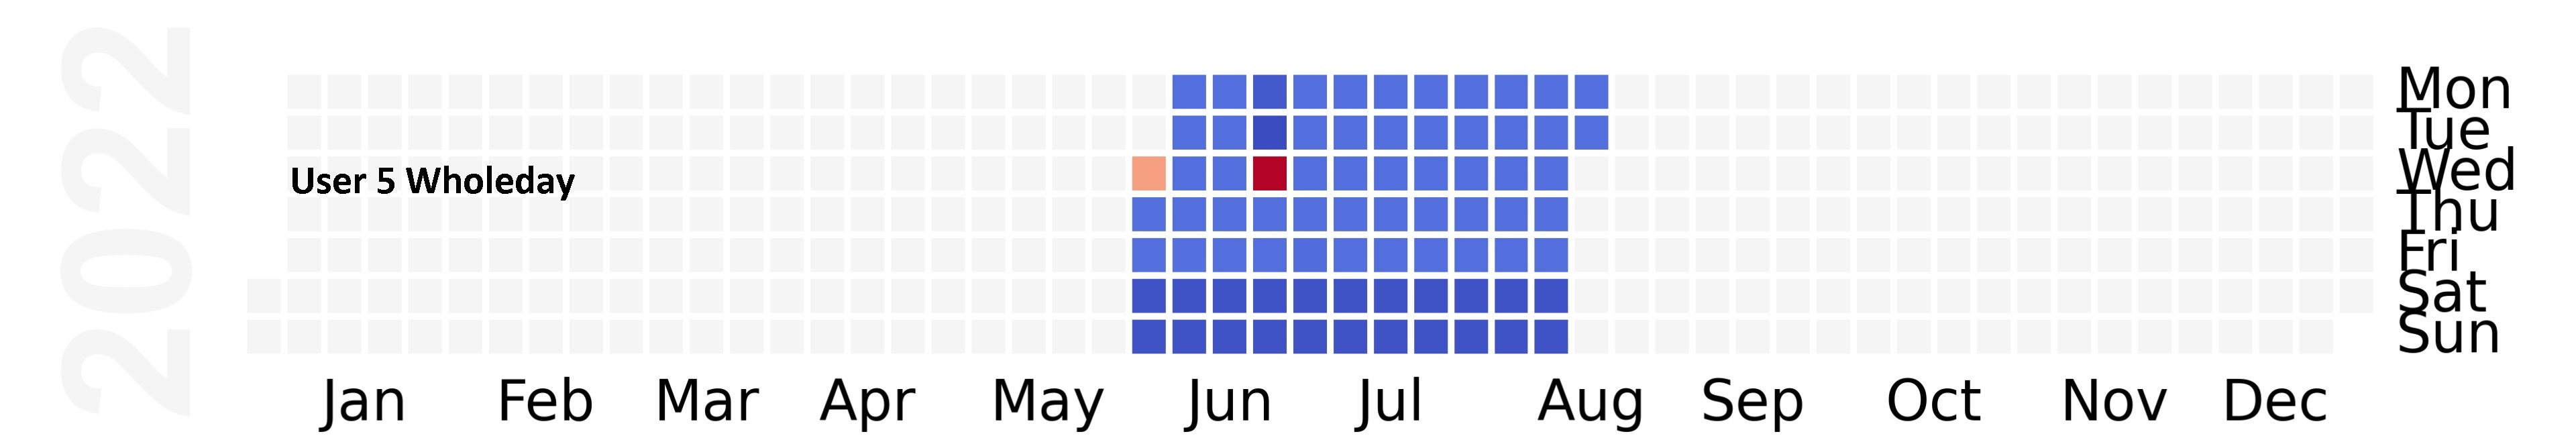
\includegraphics[width=0.5\textwidth]{images/heatmaps/user_5_wholeday_cal.png}}
    \subfloat{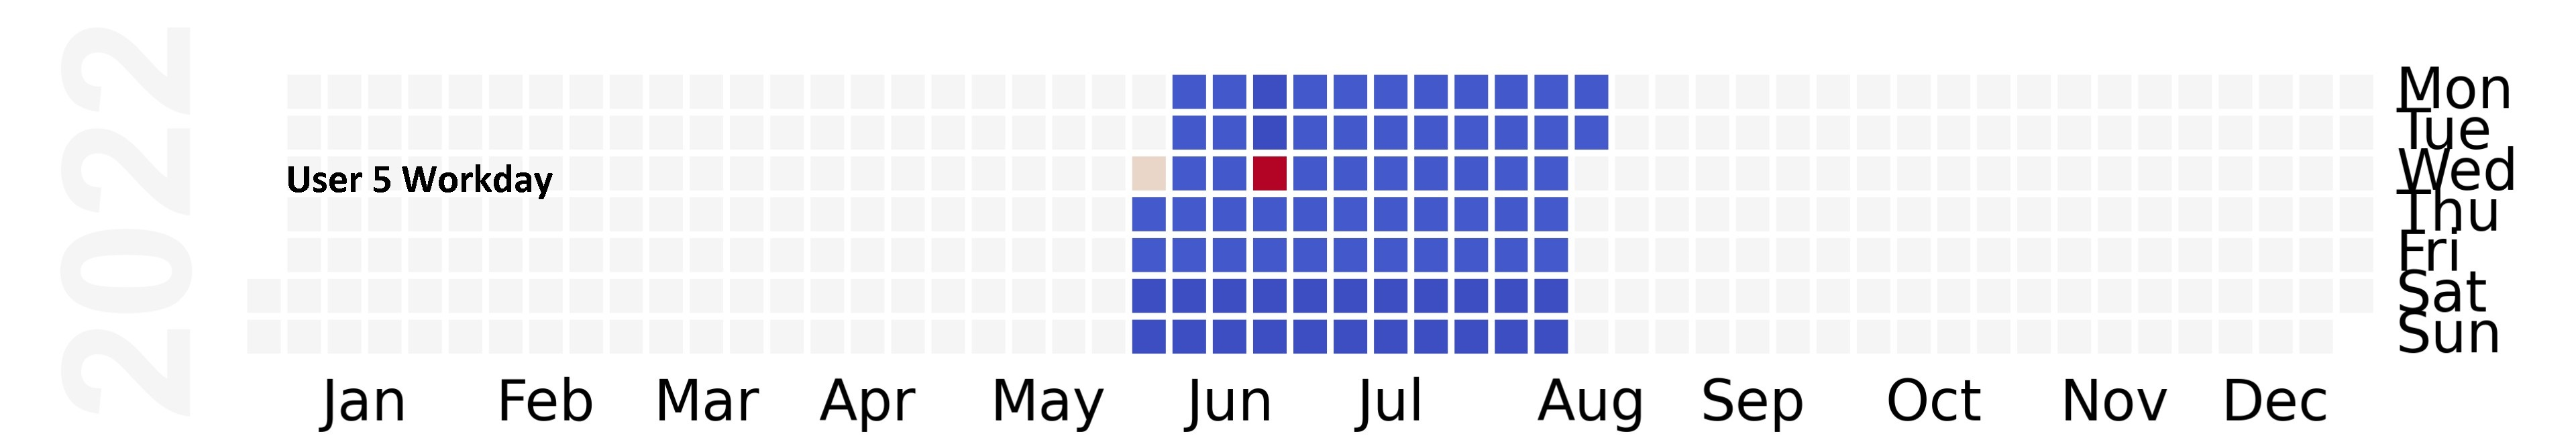
\includegraphics[width=0.5\textwidth]{images/heatmaps/user_5_workday_cal.png}}\newline
    \subfloat{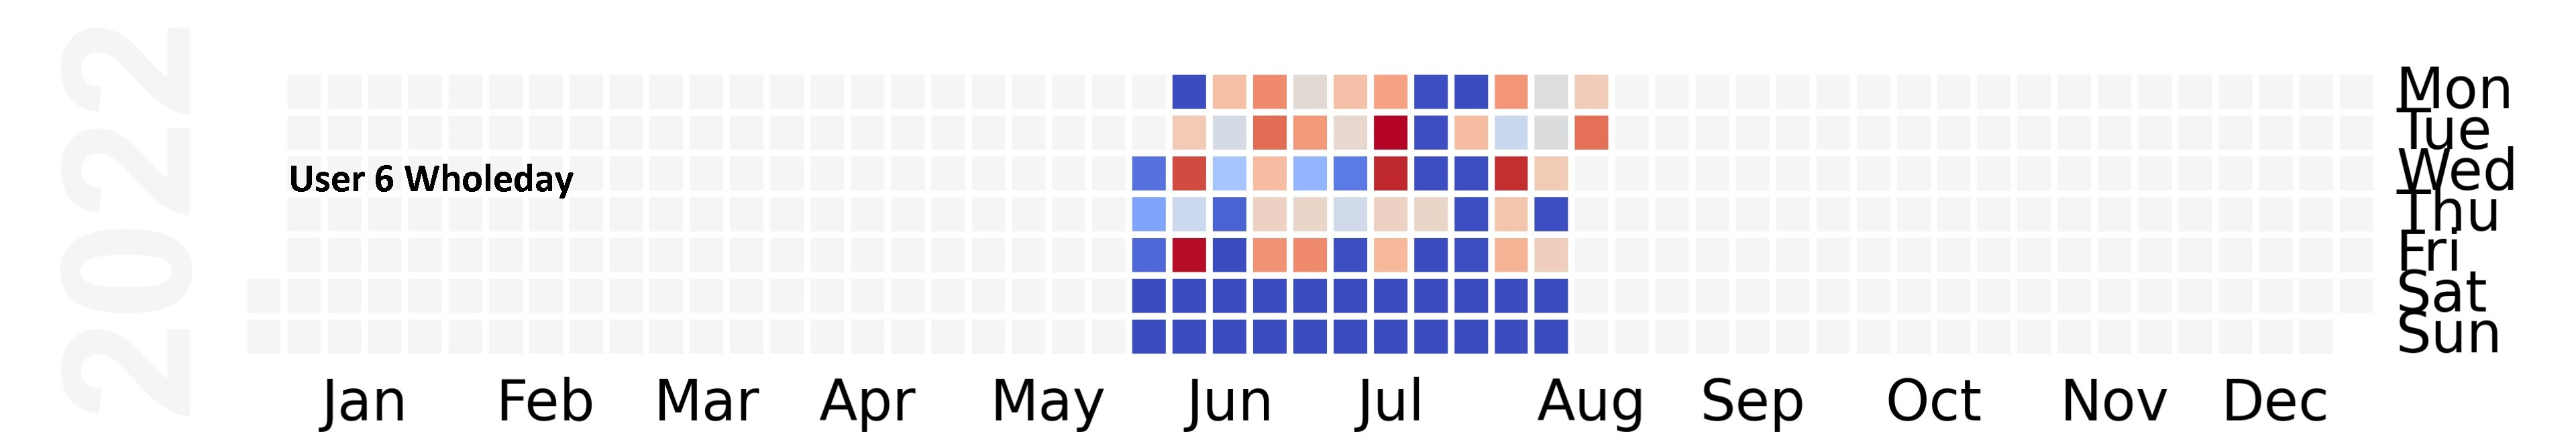
\includegraphics[width=0.5\textwidth]{images/heatmaps/user_6_wholeday_cal.png}}
    \subfloat{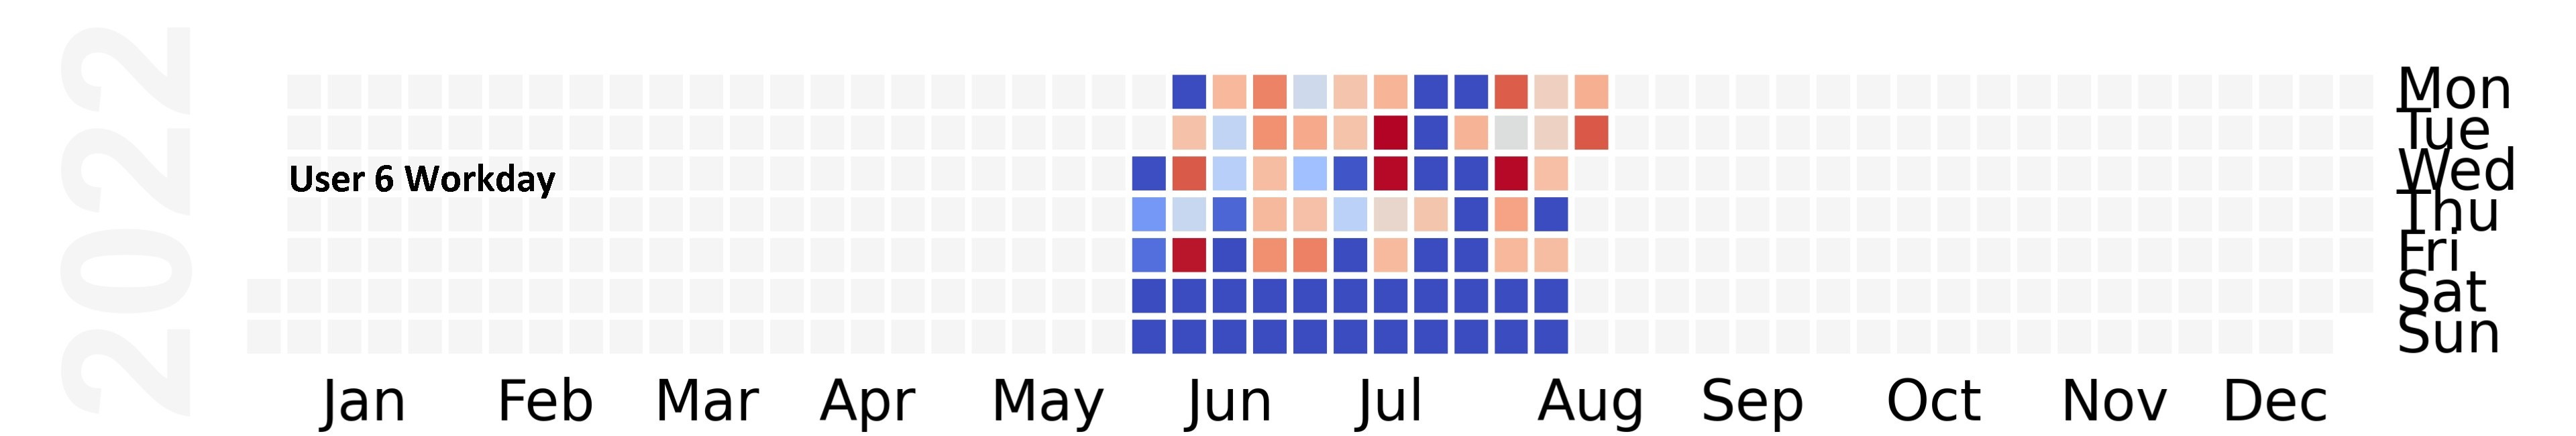
\includegraphics[width=0.5\textwidth]{images/heatmaps/user_6_workday_cal.png}}\newline
        \subfloat{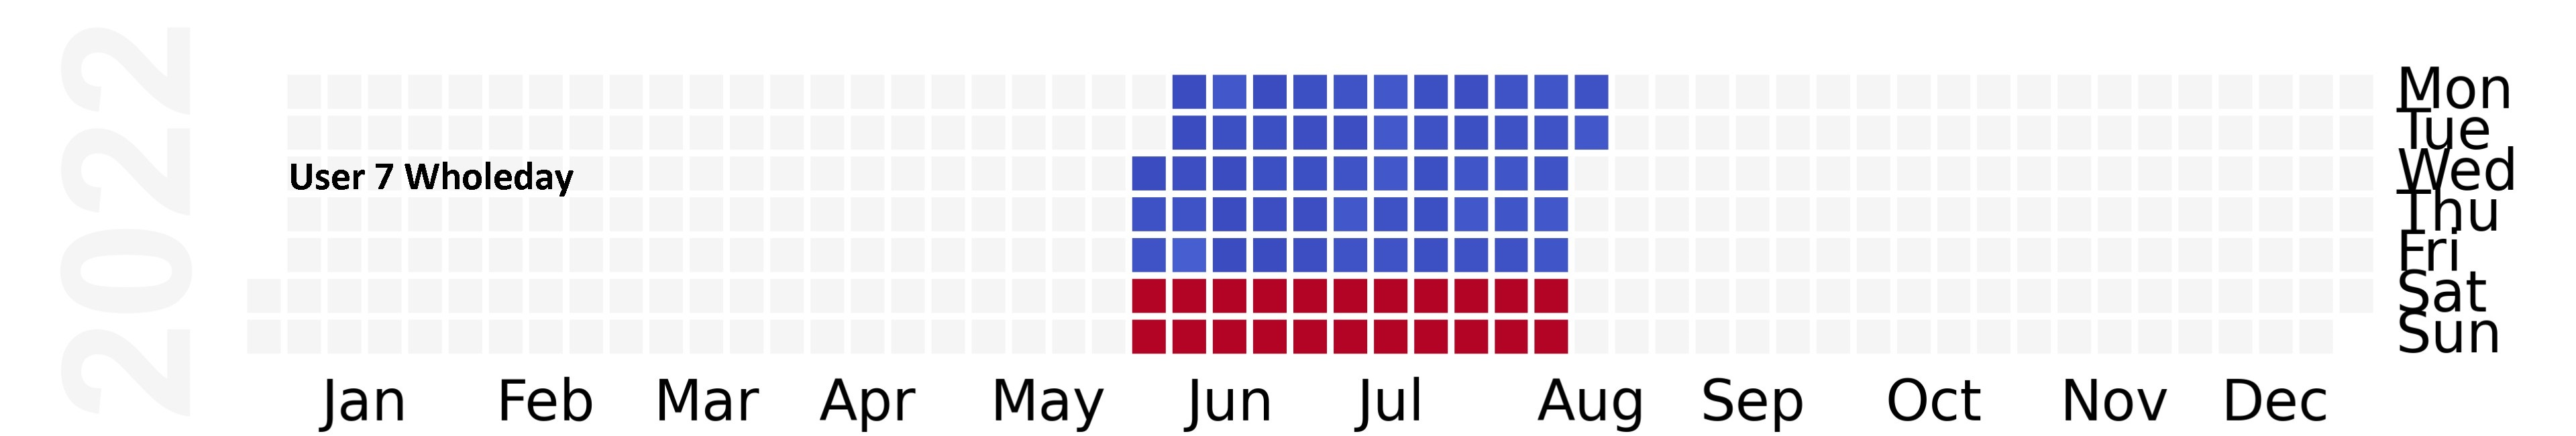
\includegraphics[width=0.5\textwidth]{images/heatmaps/user_7_wholeday_cal.png}}
    \subfloat{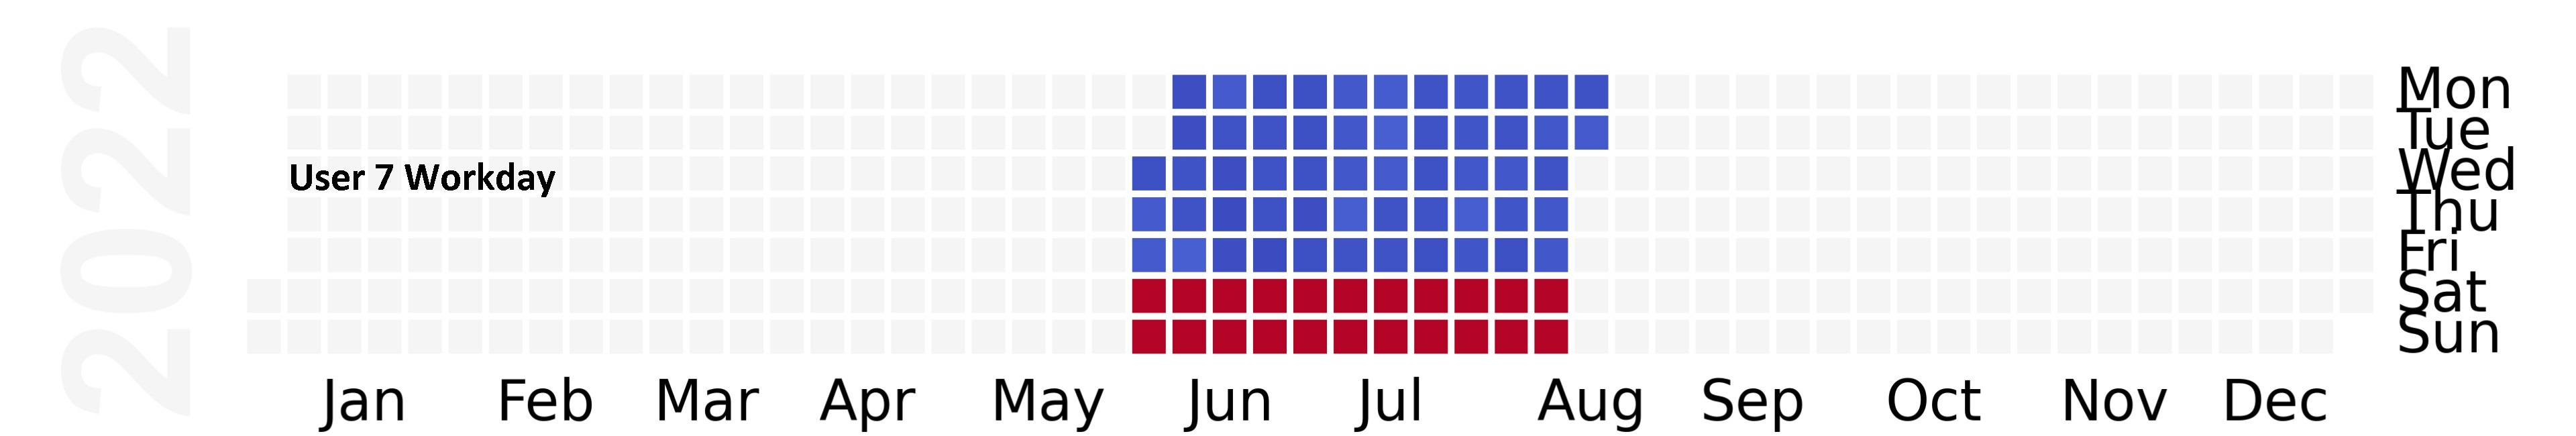
\includegraphics[width=0.5\textwidth]{images/heatmaps/user_7_workday_cal.png}}\newline
    \subfloat{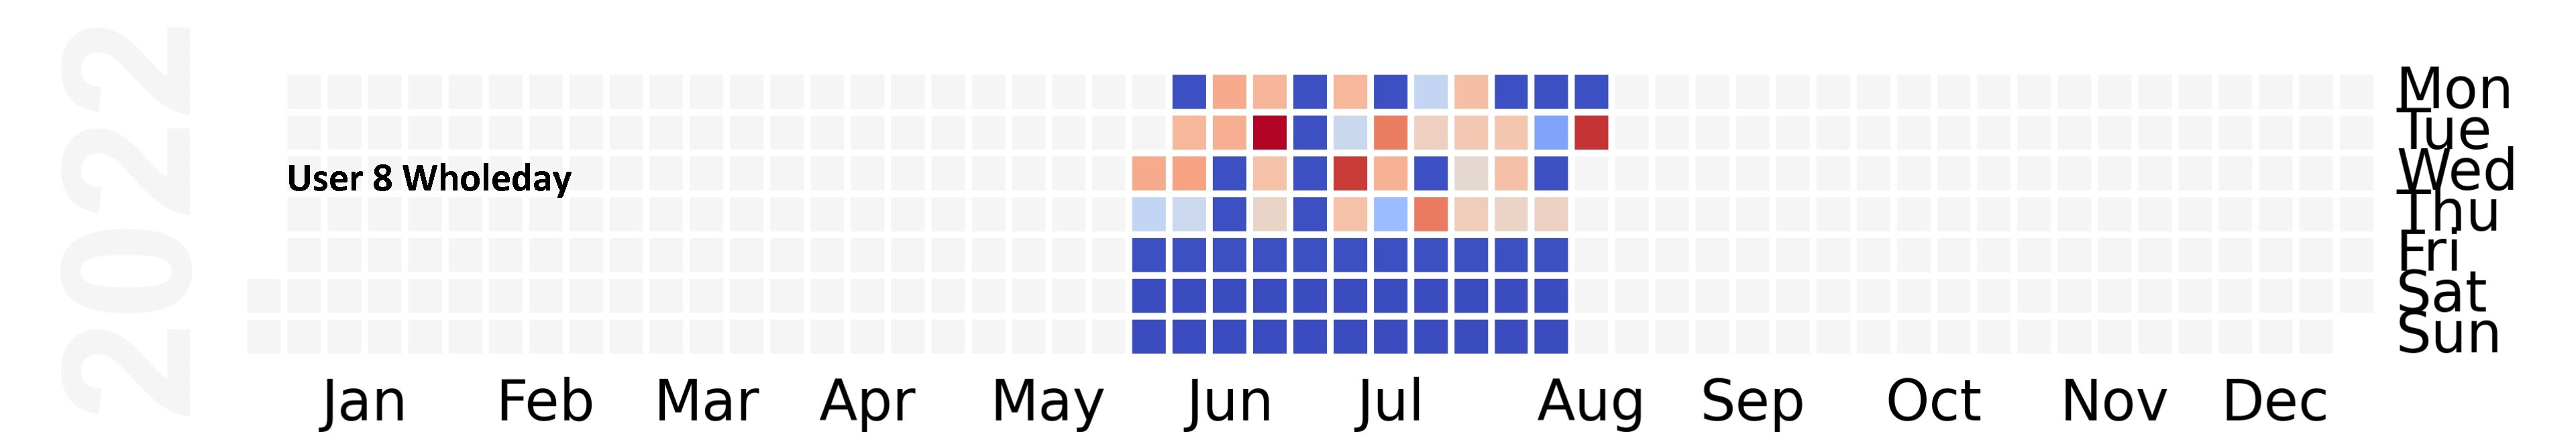
\includegraphics[width=0.5\textwidth]{images/heatmaps/user_8_wholeday_cal.png}}
    \subfloat{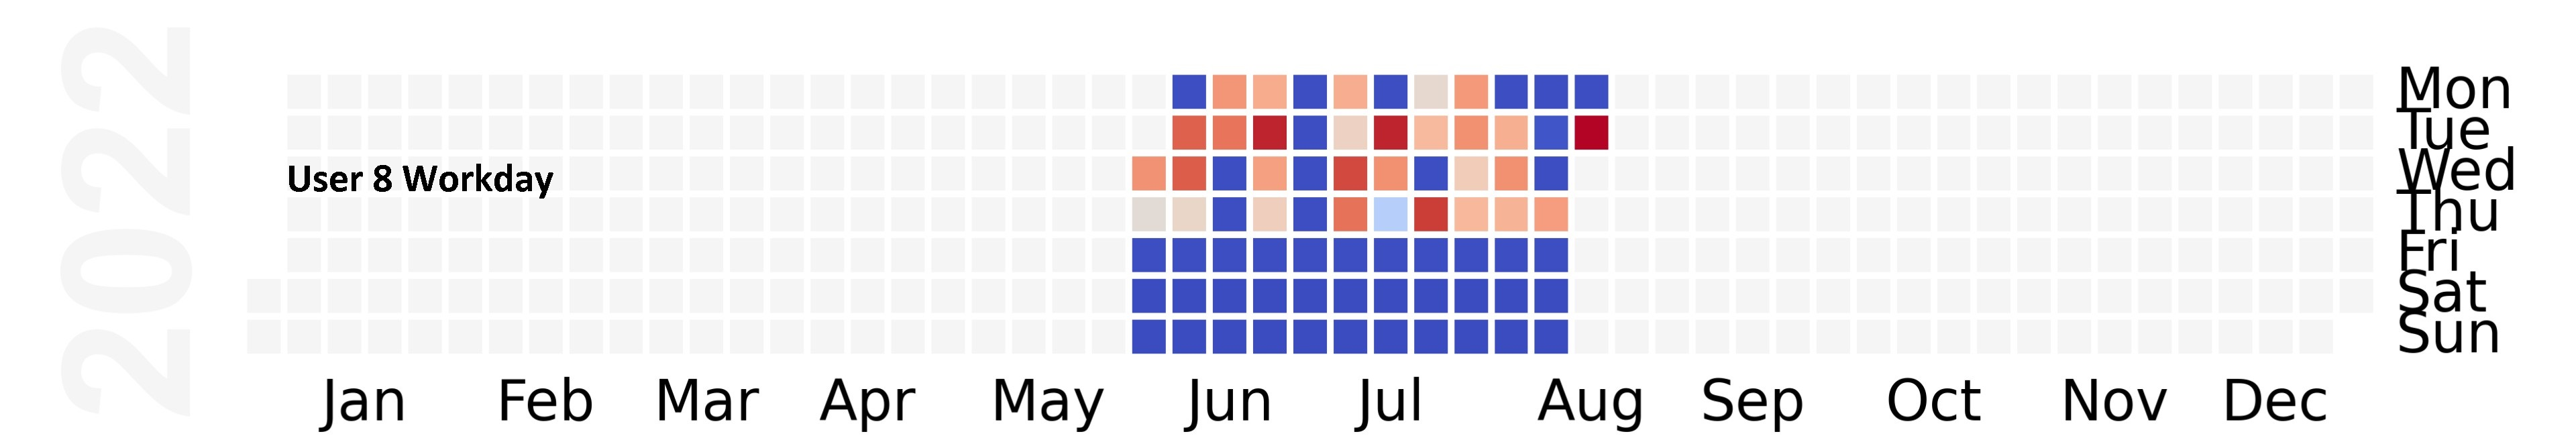
\includegraphics[width=0.5\textwidth]{images/heatmaps/user_8_workday_cal.png}}\newline
    \subfloat{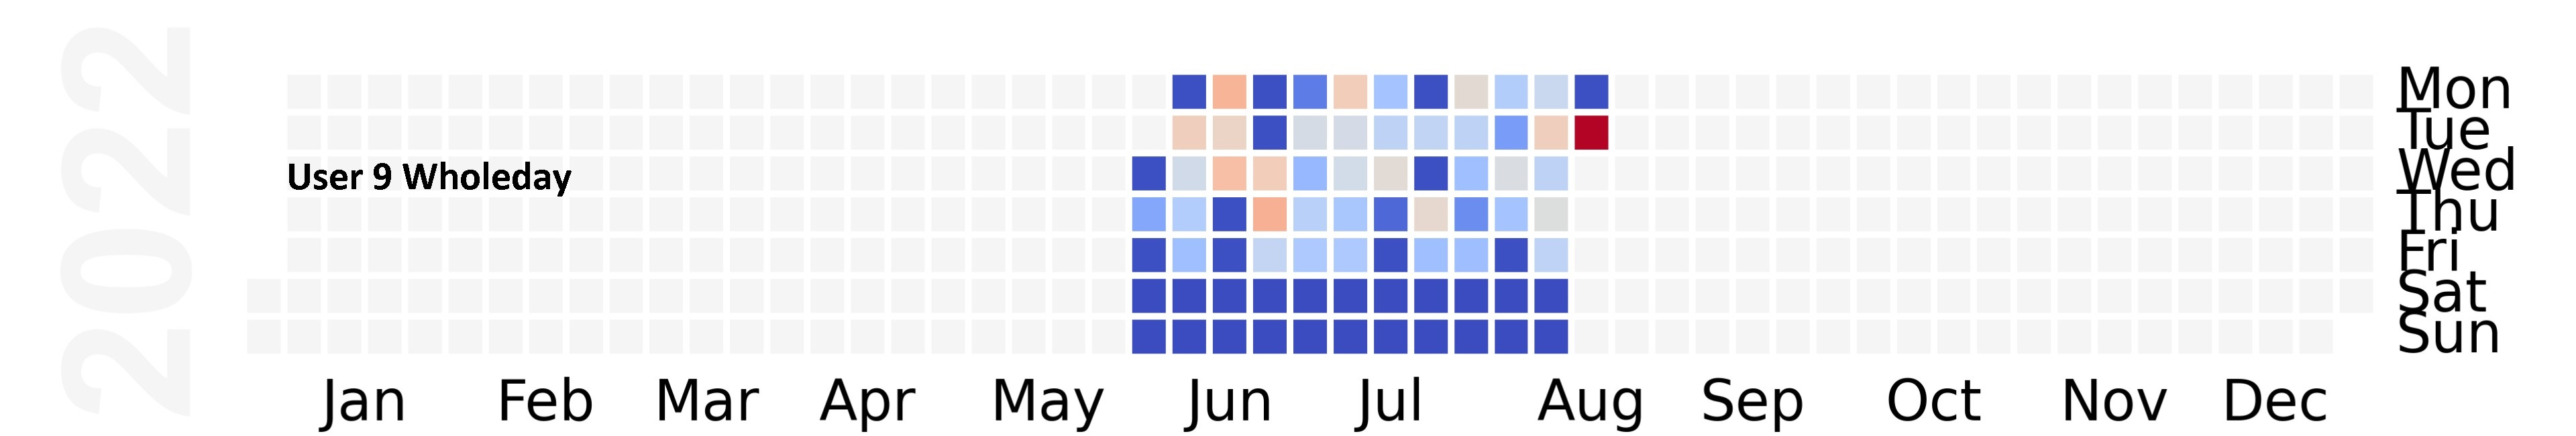
\includegraphics[width=0.5\textwidth]{images/heatmaps/user_9_wholeday_cal.png}}
    \subfloat{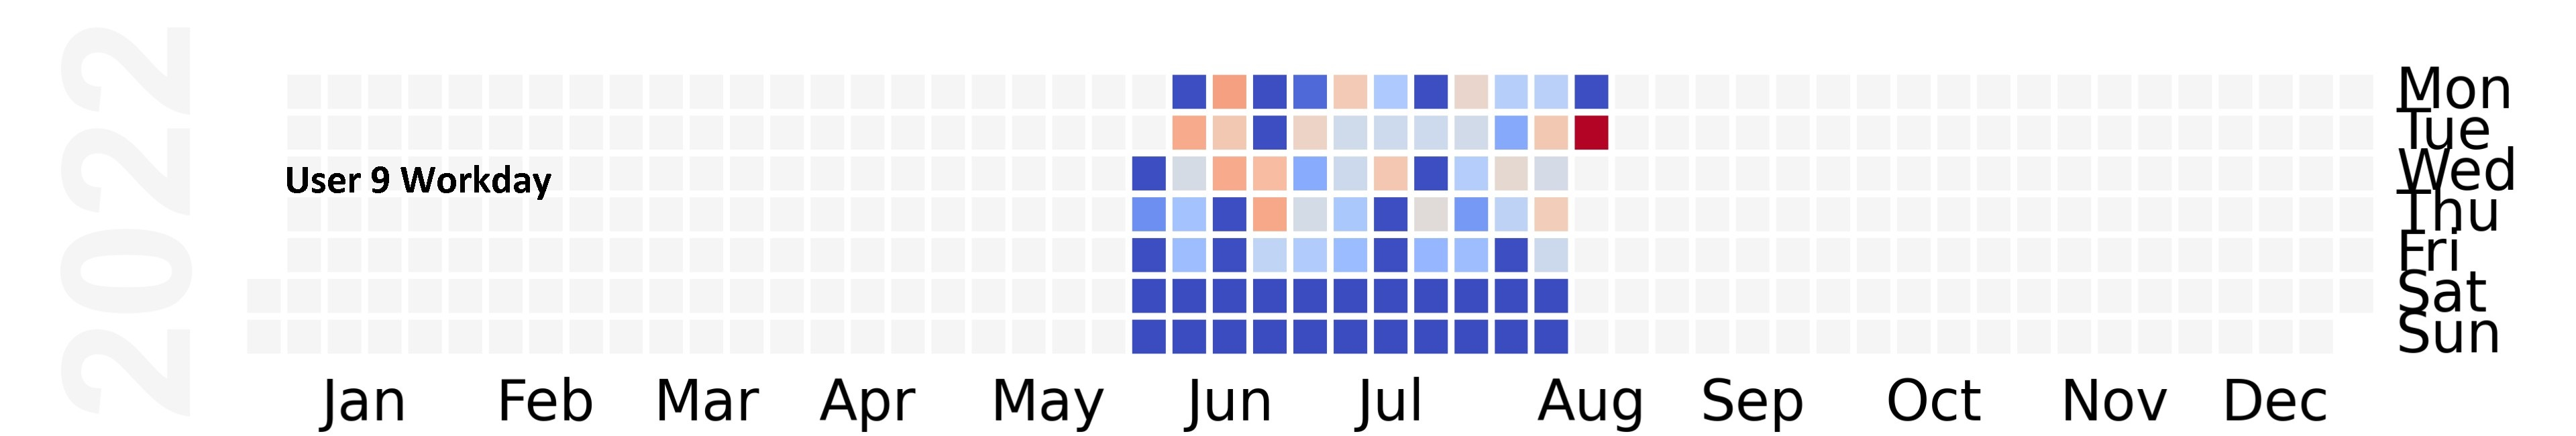
\includegraphics[width=0.5\textwidth]{images/heatmaps/user_9_workday_cal.png}}\newline
    \subfloat{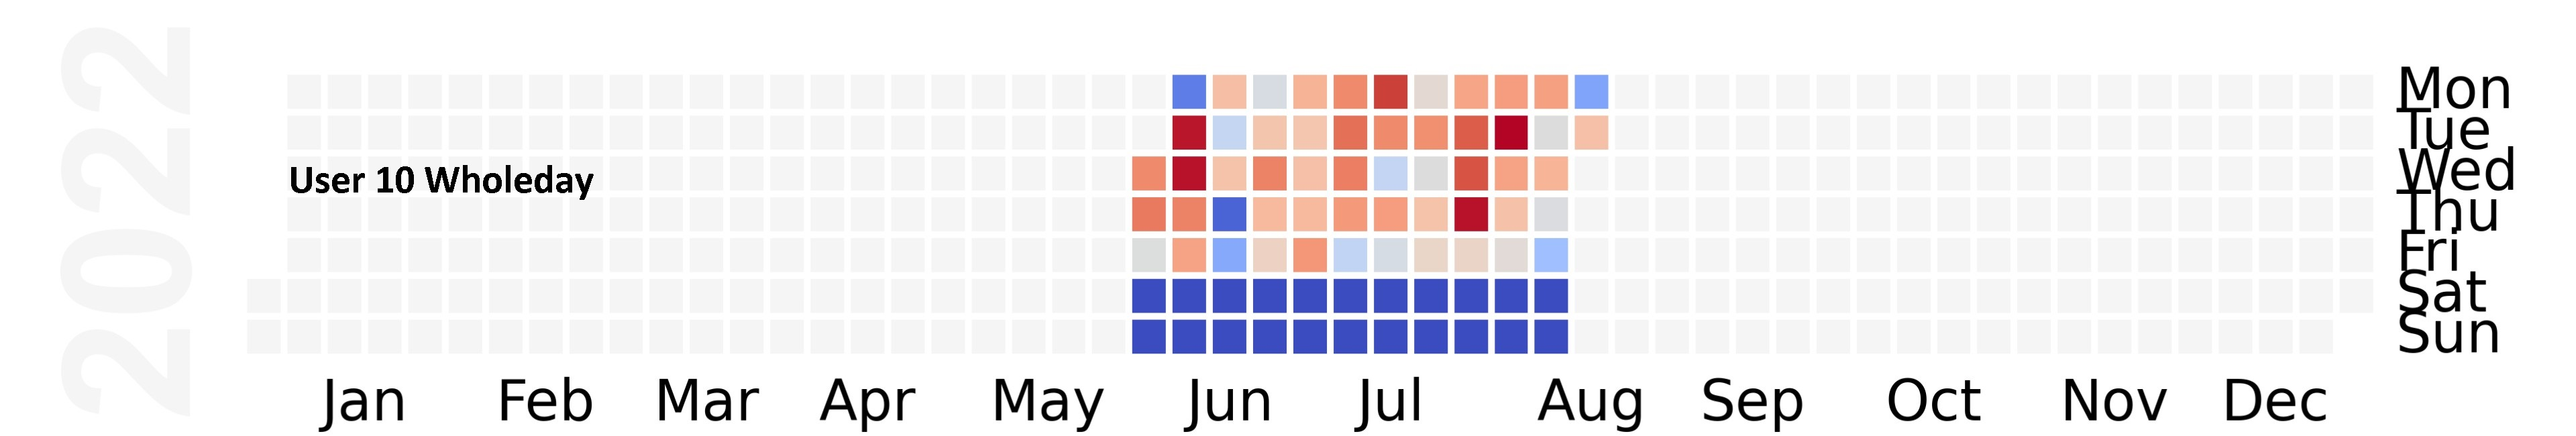
\includegraphics[width=0.5\textwidth]{images/heatmaps/user_10_wholeday_cal.png}}
    \subfloat{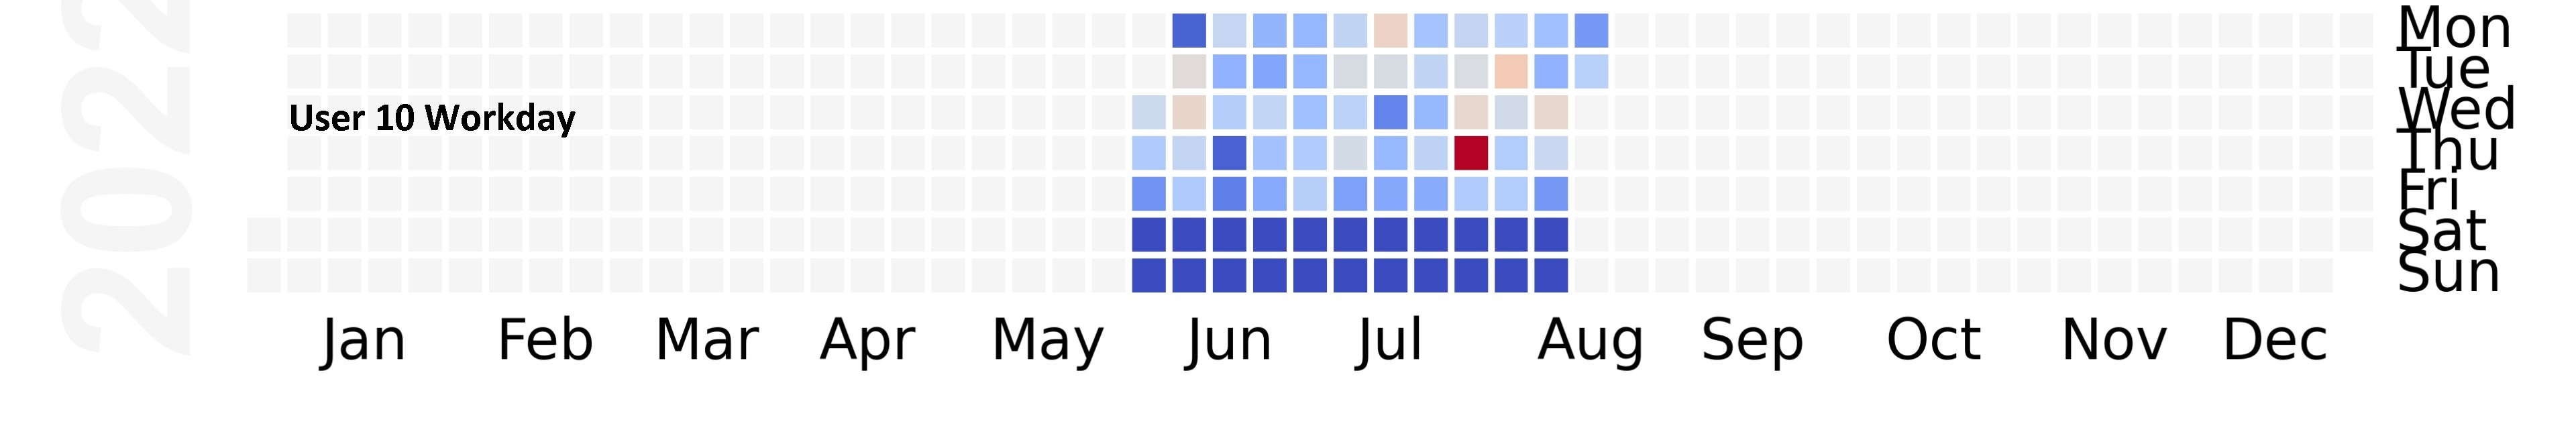
\includegraphics[width=0.5\textwidth]{images/heatmaps/user_10_workday_cal.png}}\newline
    \subfloat{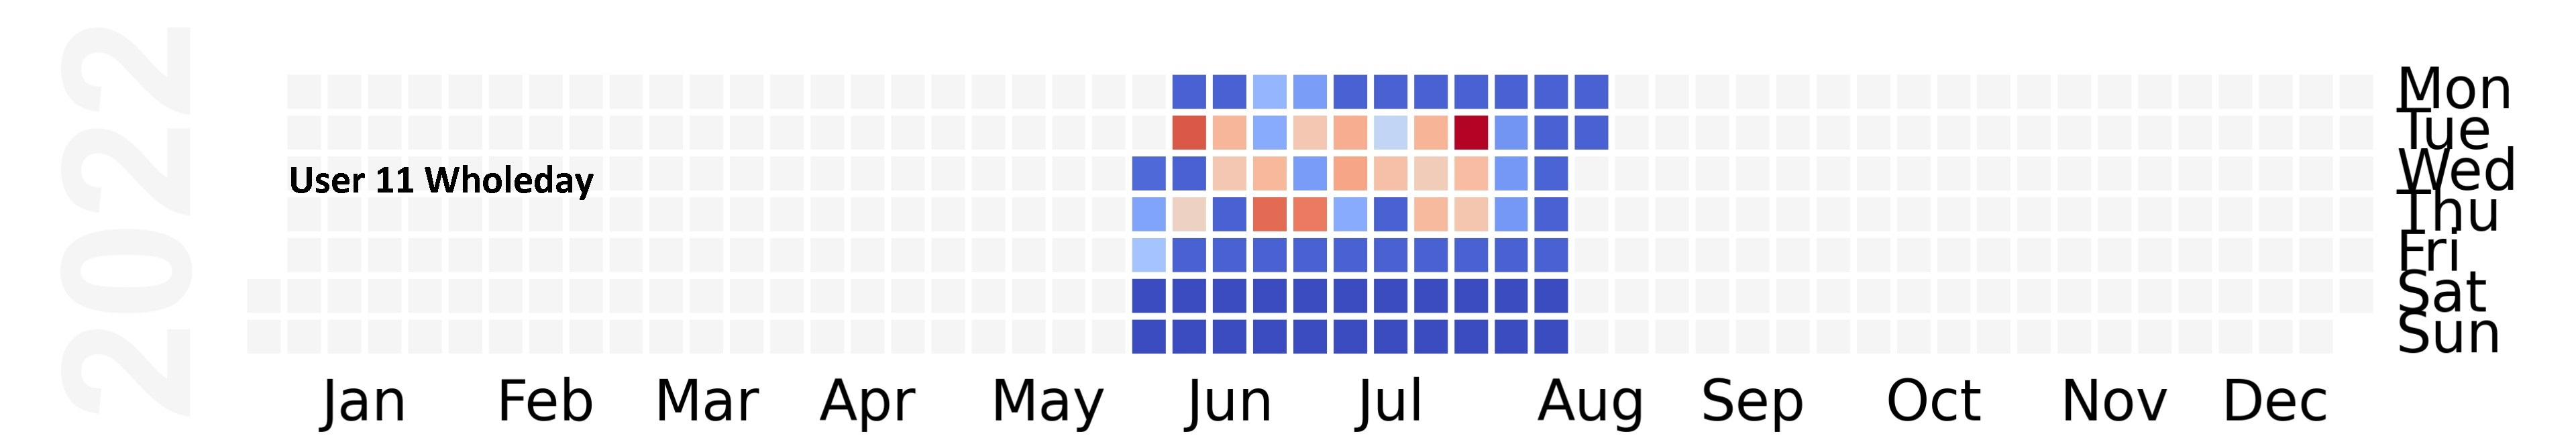
\includegraphics[width=0.5\textwidth]{images/heatmaps/user_11_wholeday_cal.png}}
    \subfloat{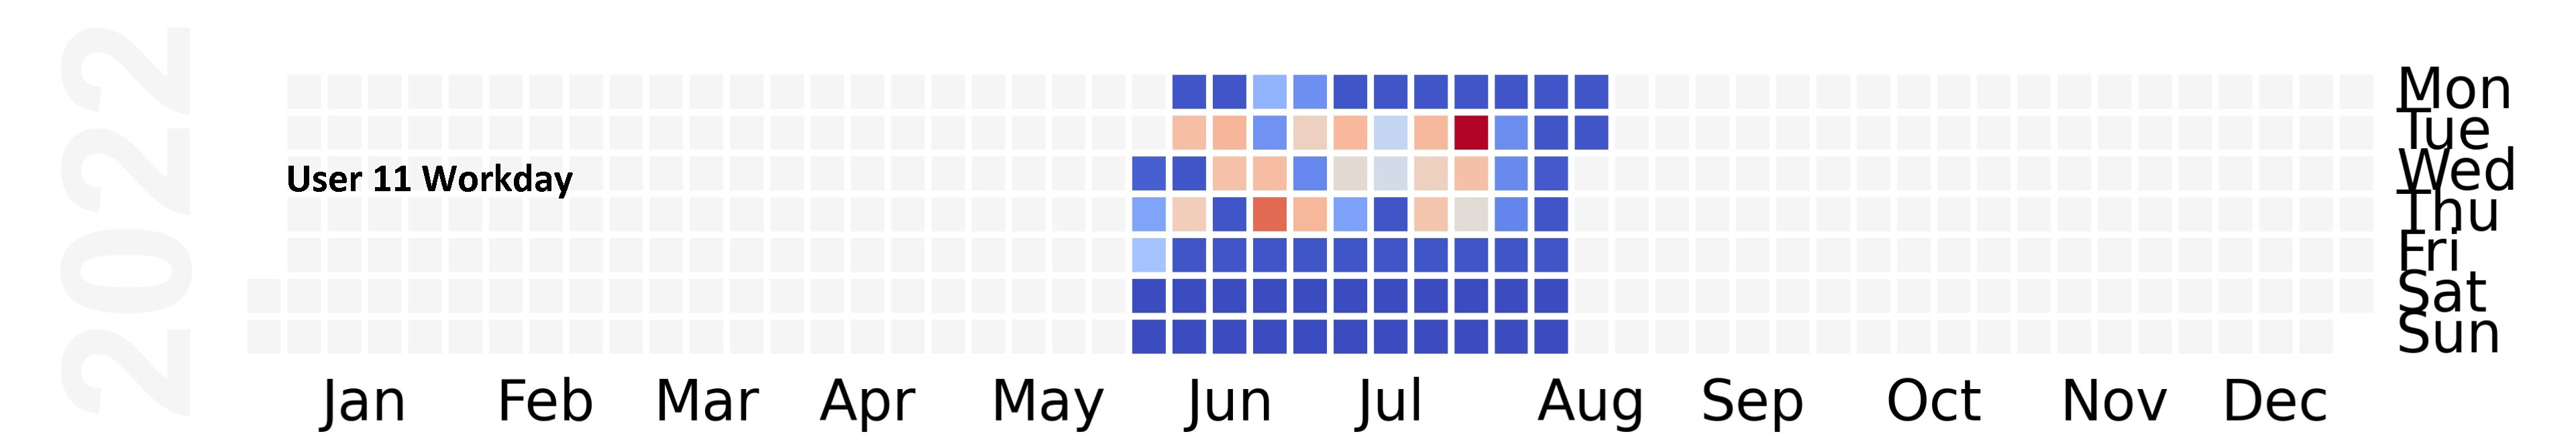
\includegraphics[width=0.5\textwidth]{images/heatmaps/user_11_workday_cal.png}}\newline
    \subfloat{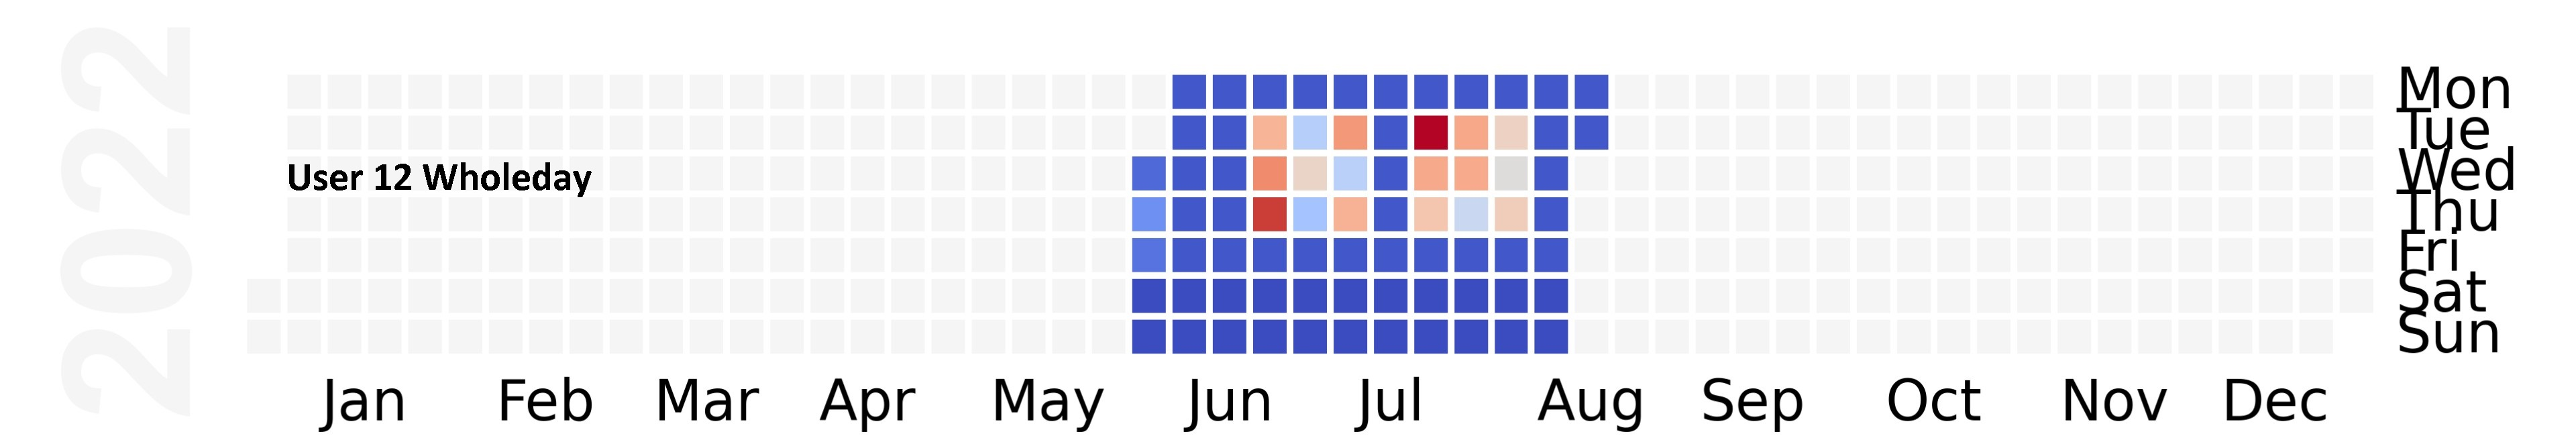
\includegraphics[width=0.5\textwidth]{images/heatmaps/user_12_wholeday_cal.png}}
    \subfloat{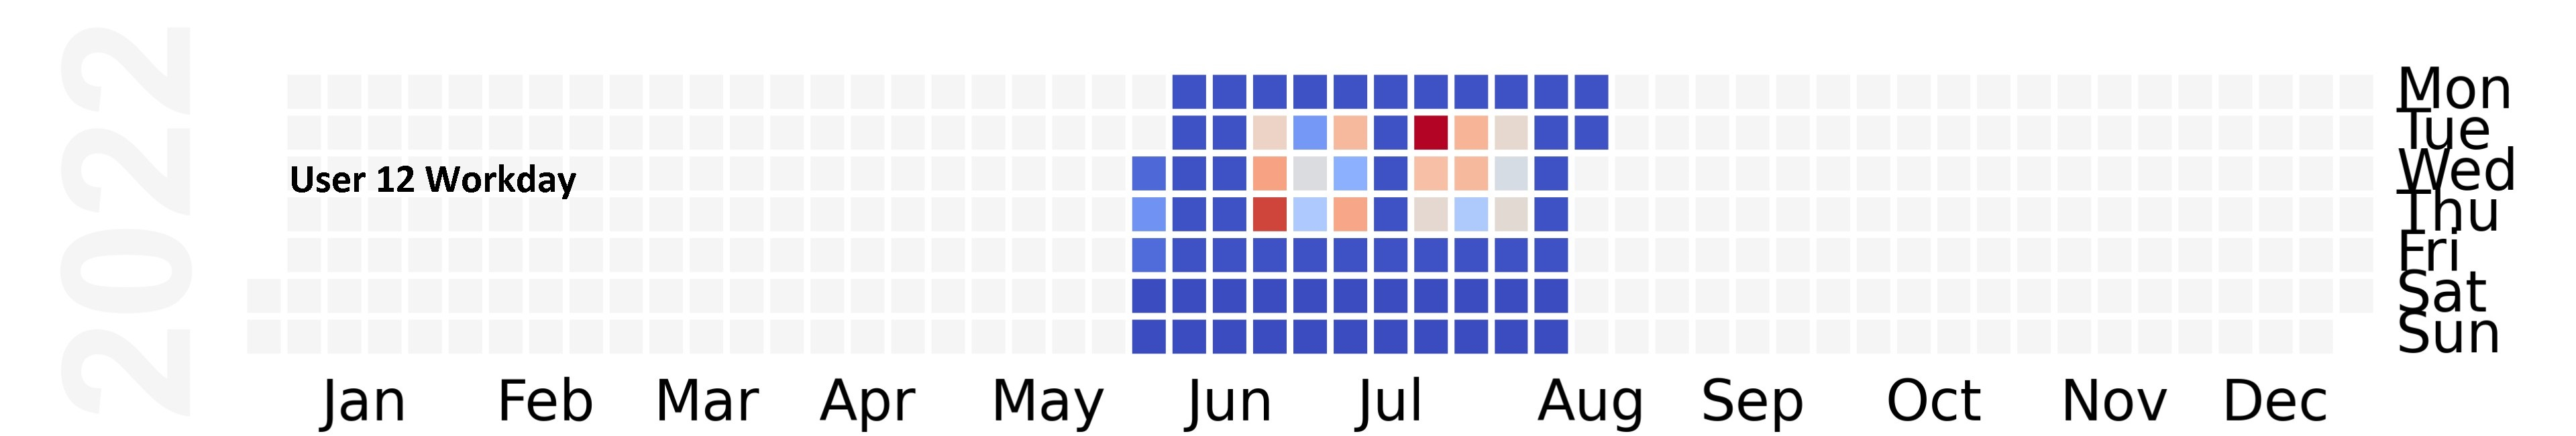
\includegraphics[width=0.5\textwidth]{images/heatmaps/user_12_workday_cal.png}}\newline
    \subfloat{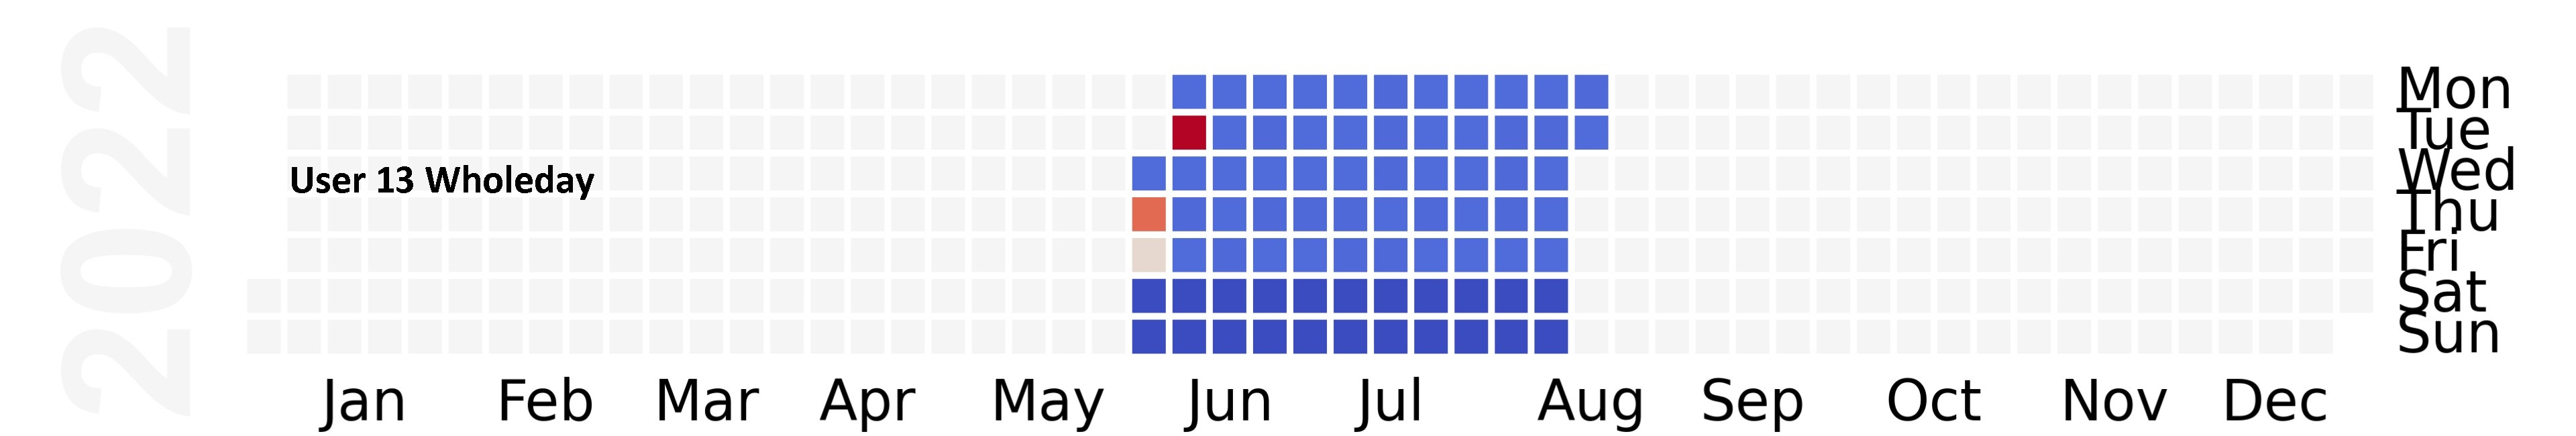
\includegraphics[width=0.5\textwidth]{images/heatmaps/user_13_wholeday_cal.png}}
    \subfloat{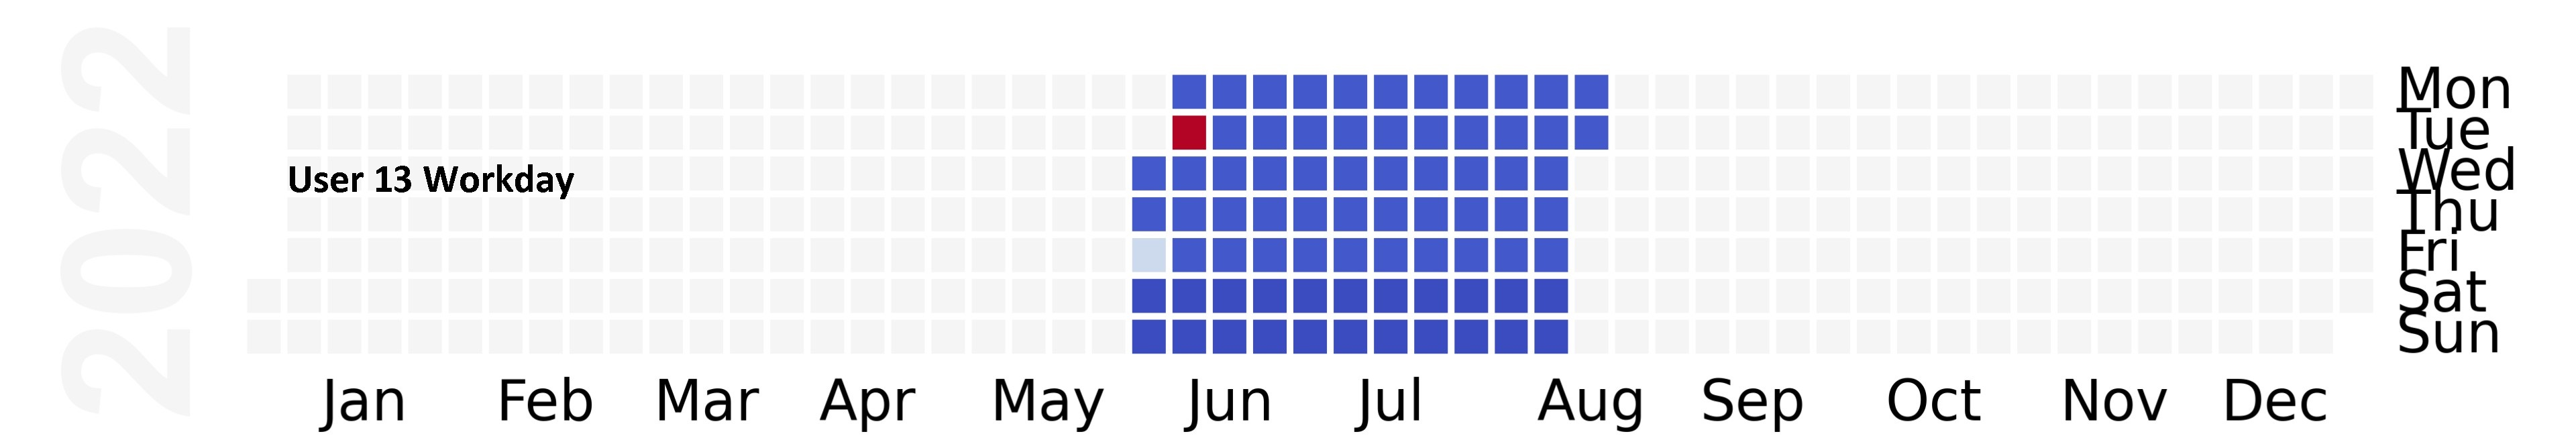
\includegraphics[width=0.5\textwidth]{images/heatmaps/user_13_workday_cal.png}}\newline
    \subfloat{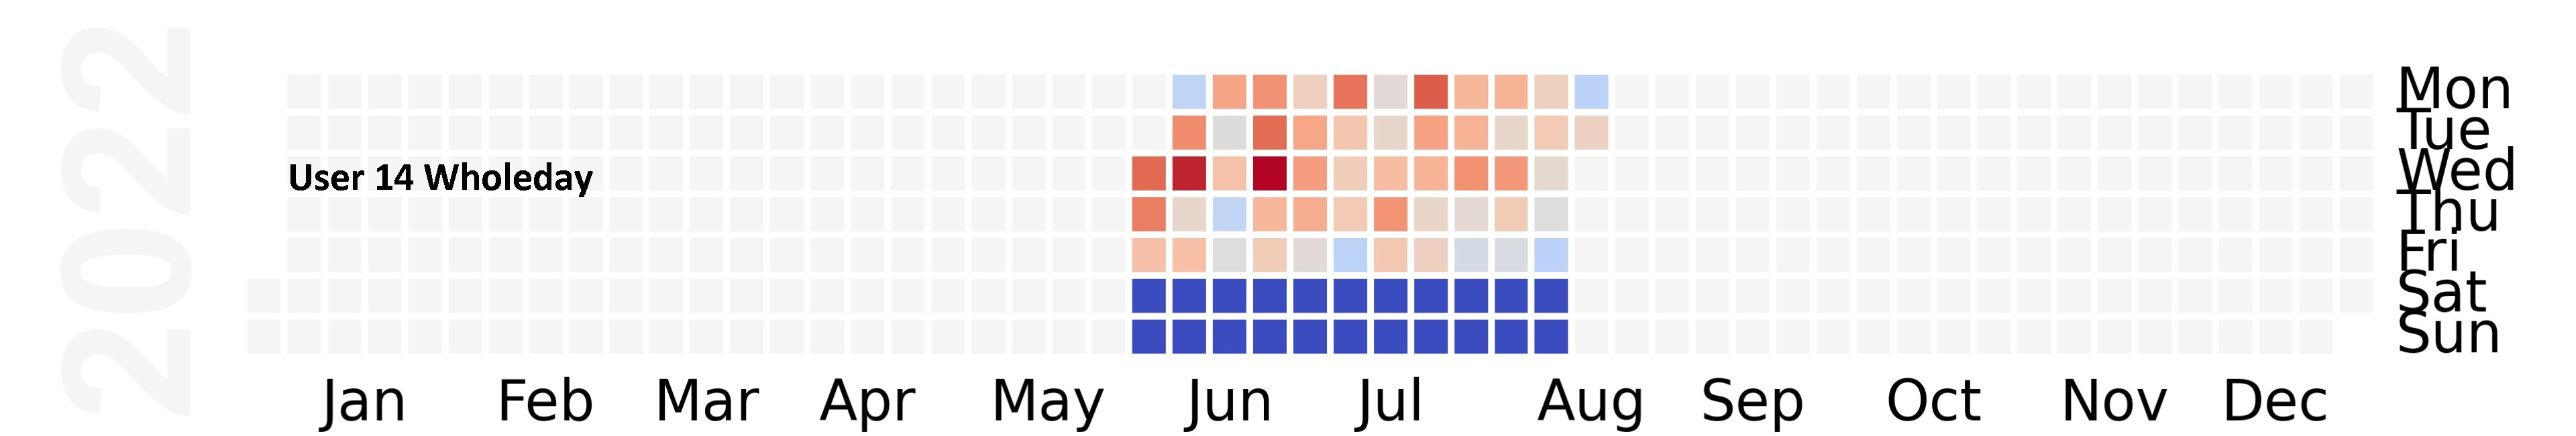
\includegraphics[width=0.5\textwidth]{images/heatmaps/user_14_wholeday_cal.png}}
    \subfloat{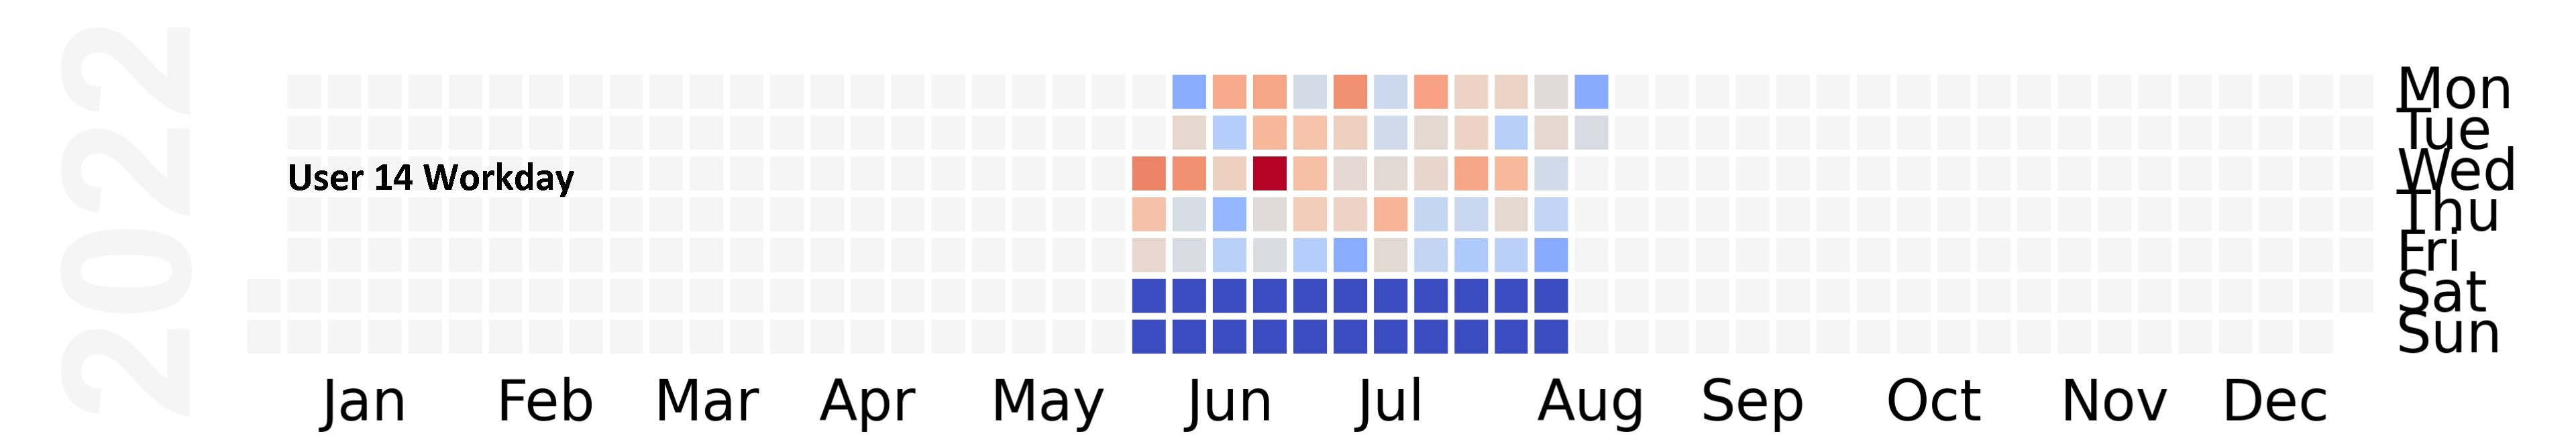
\includegraphics[width=0.5\textwidth]{images/heatmaps/user_14_workday_cal.png}}\newline
    \subfloat{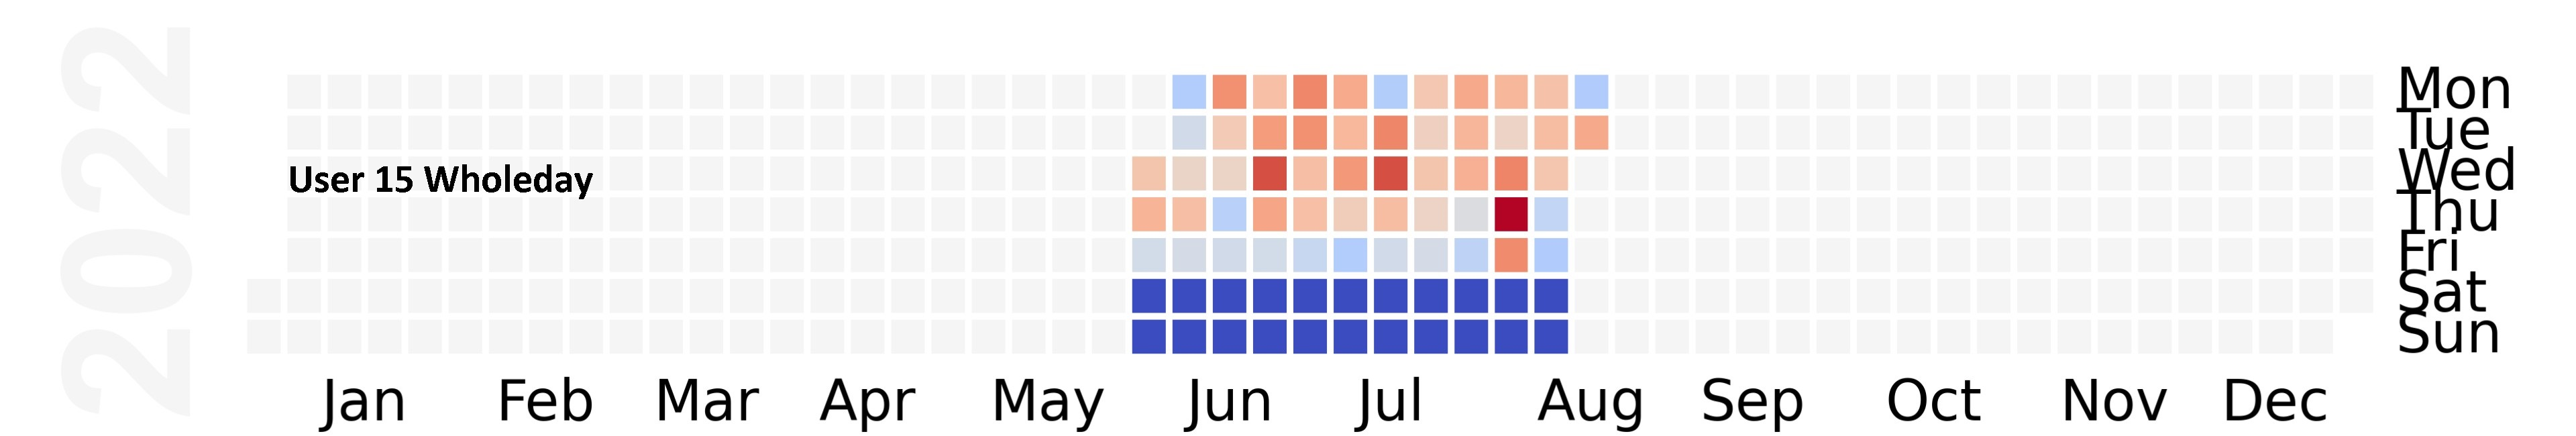
\includegraphics[width=0.5\textwidth]{images/heatmaps/user_15_wholeday_cal.png}}
    \subfloat{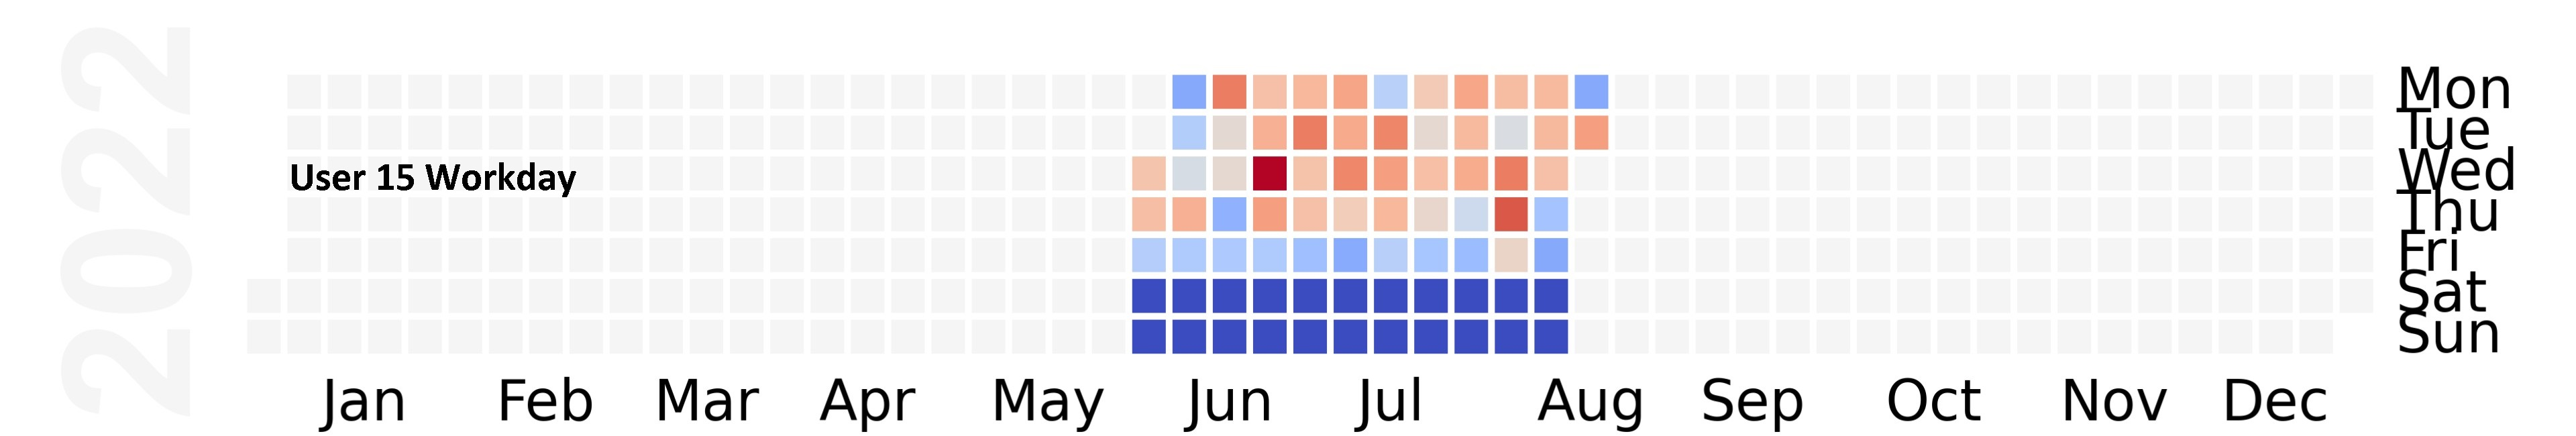
\includegraphics[width=0.5\textwidth]{images/heatmaps/user_15_workday_cal.png}}\newline
    \caption{\centering Comparison of the consumption of each user (Row 1-15) over time. Consumption is only considered without weekends with averages during the weekday (left) and working hours (right).}
    \label{fig:user_comparison}
\end{figure}
\noindent The observation of reduced consumption on Fridays is increasingly clear using the illustration in figure \ref{fig:office_consumption}. The increased attendance on Wednesday in calendar week 25, as well as Tuesday in the last week is clearly distinguishable. By comparing single user heat maps to the summation can show differentiation between quantitative consumption peaks (consumption due to a higher amount of people) and qualitative peaks (high spikes in consumption due to changes in the workload/ type of labor).
\begin{figure}[ht]
	\centering
	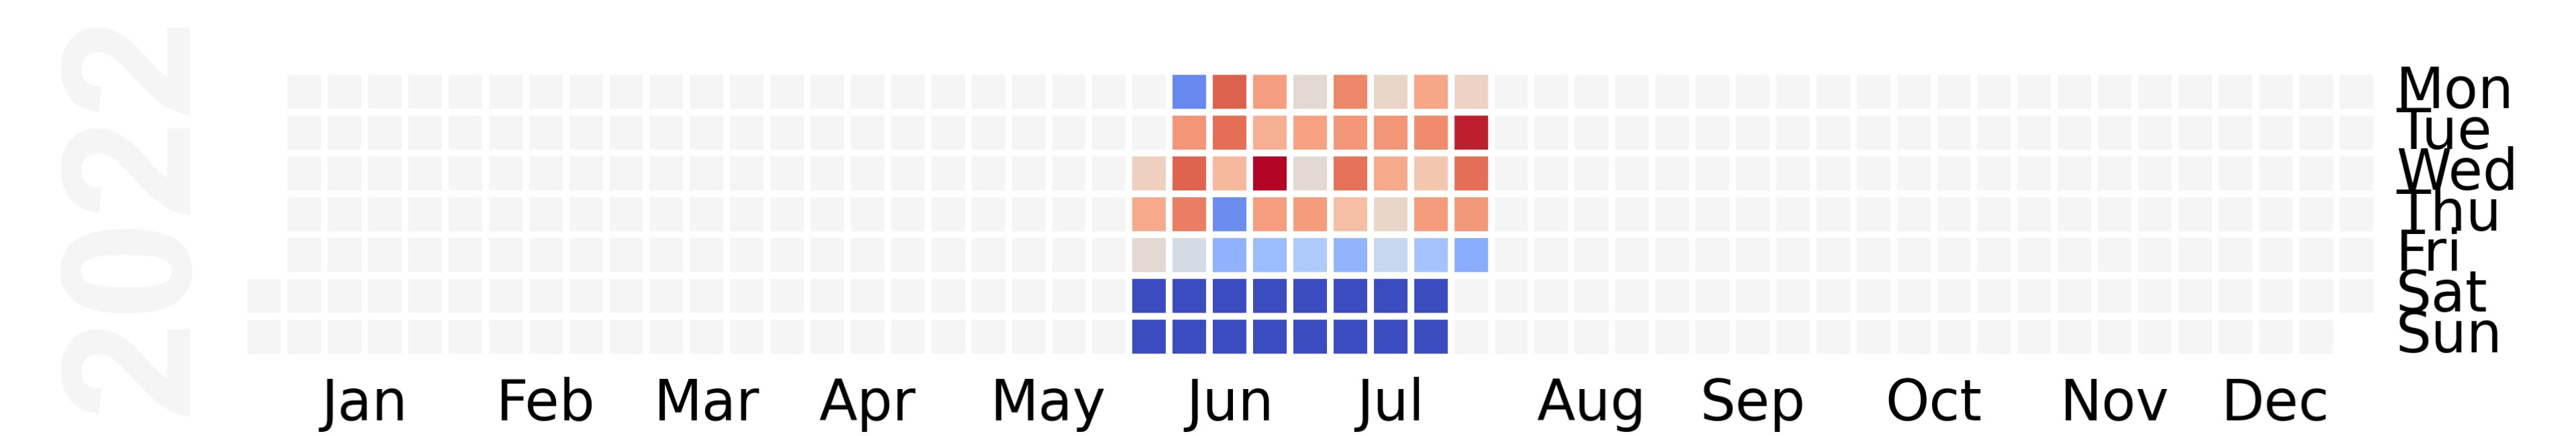
\includegraphics[width=\textwidth]{images/heatmaps/workday_cal.png}
	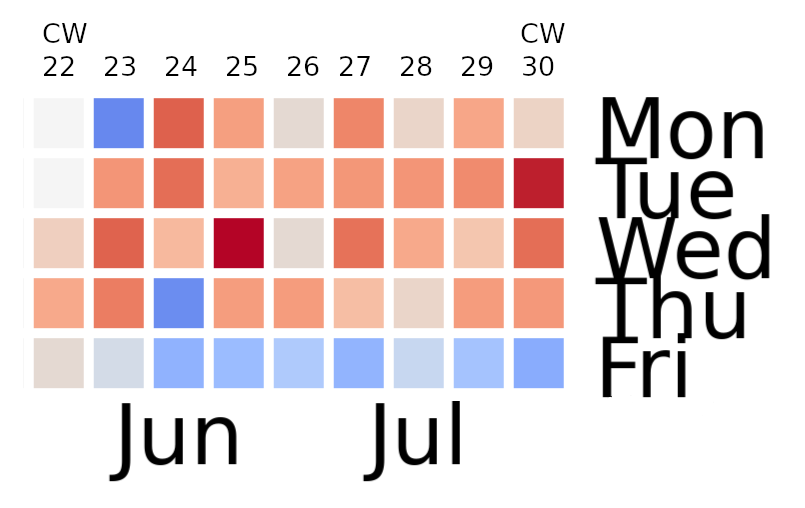
\includegraphics[width=\textwidth]{workday_cal_edit2.png}
	\caption{Heat map of the sum of all sensors during usual office hours (work hours on \glspl{workday}).Above the unedited plot, below an edited version to improve visibility.}
	\label{fig:office_consumption}
\end{figure}
\begin{figure}[ht]
	\centering
	Personal Computers
	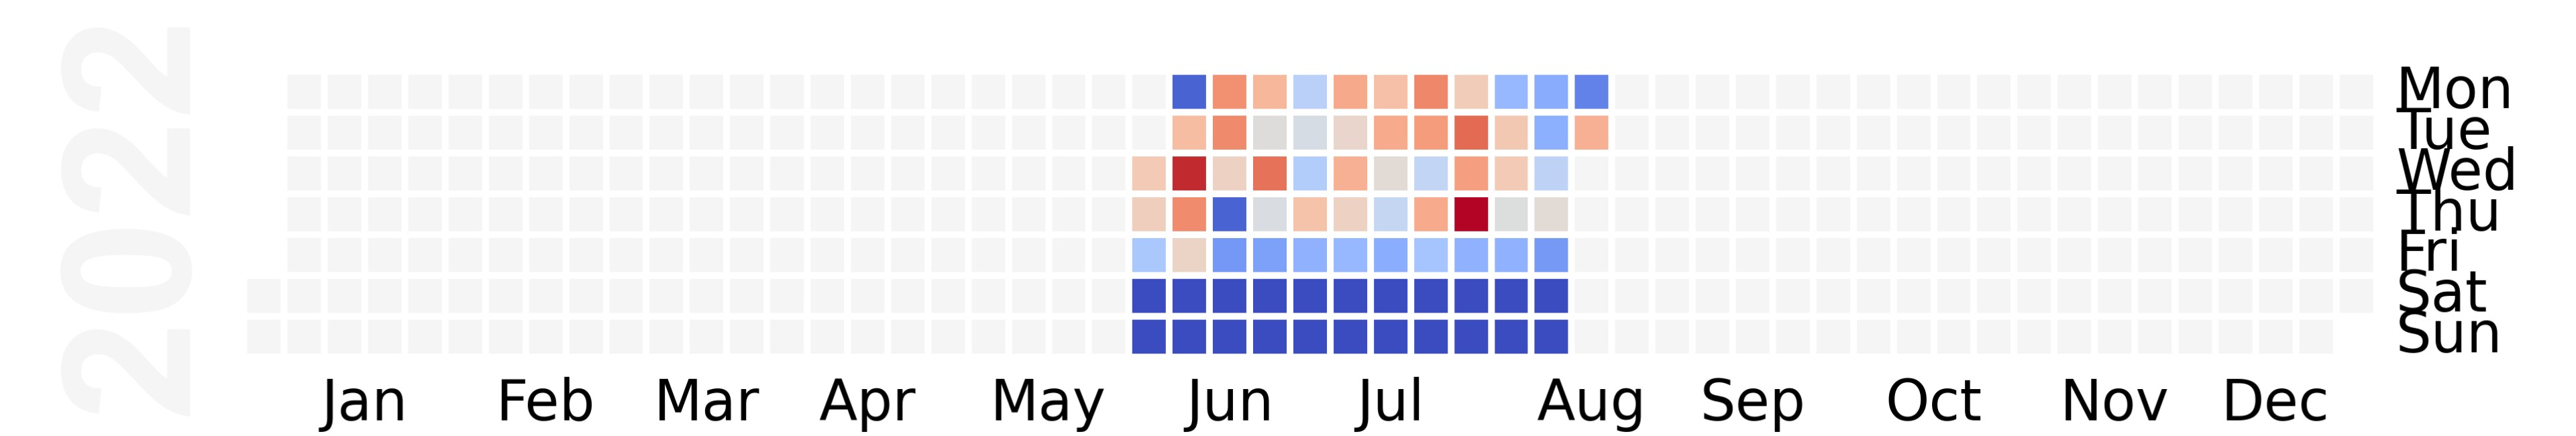
\includegraphics[width=\textwidth]{images/heatmaps/devicetype_PC_workday_cal.png}
	\caption{Heat map of the sum of all PC sensors during usual office hours (measured during \glspl{workday}).}
	\label{fig:pc_hm}
\end{figure}
\noindent As expected the consumption patterns of Monitors highly correlate the pattern given by PC measurements, which can be compared using figures \ref{fig:pc_hm} and \ref{fig:mon_hm}. In comparison the consumptions of utility devices and printer do not match nearly as neatly. In the case of printers the differentiation is harder due to the pronounced consumtpion spike on Wednesday of CW 27.
\begin{figure}[ht]
	\centering
	Monitors
	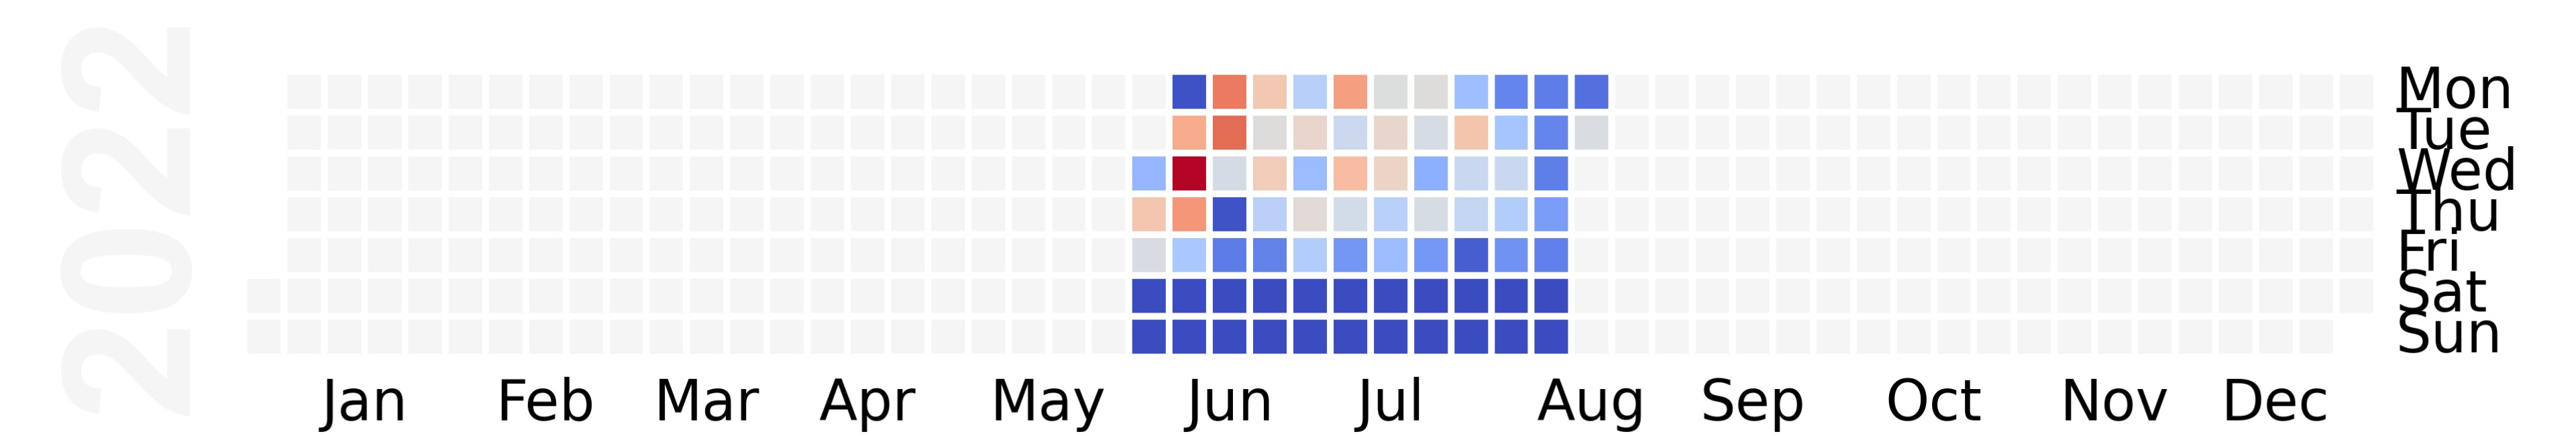
\includegraphics[width=\textwidth]{images/heatmaps/devicetype_Monitor_workday_cal.png}
	\caption{Heat map of the sum of all monitor sensors during usual office hours (measured during \glspl{workday}).}
	\label{fig:mon_hm}
\end{figure}
\begin{figure}[ht]
	\centering
	Printer
	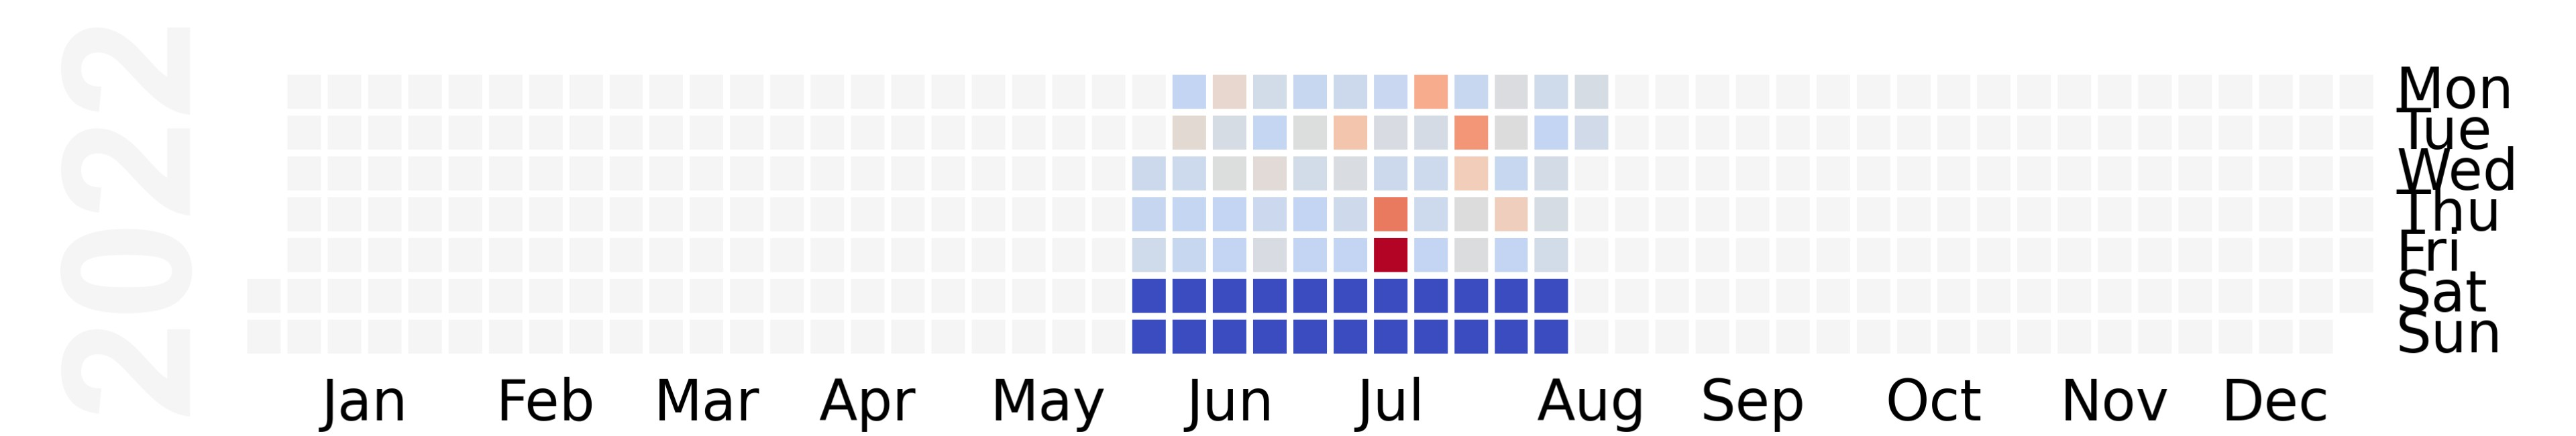
\includegraphics[width=\textwidth]{images/heatmaps/devicetype_Printer_workday_cal.png}
	\caption{Heat map of the sum of all printer sensors during usual office hours (measured during \glspl{workday}).}
	\label{fig:printer_hm}
\end{figure}

\begin{figure}[ht]
	\centering
	Utilities	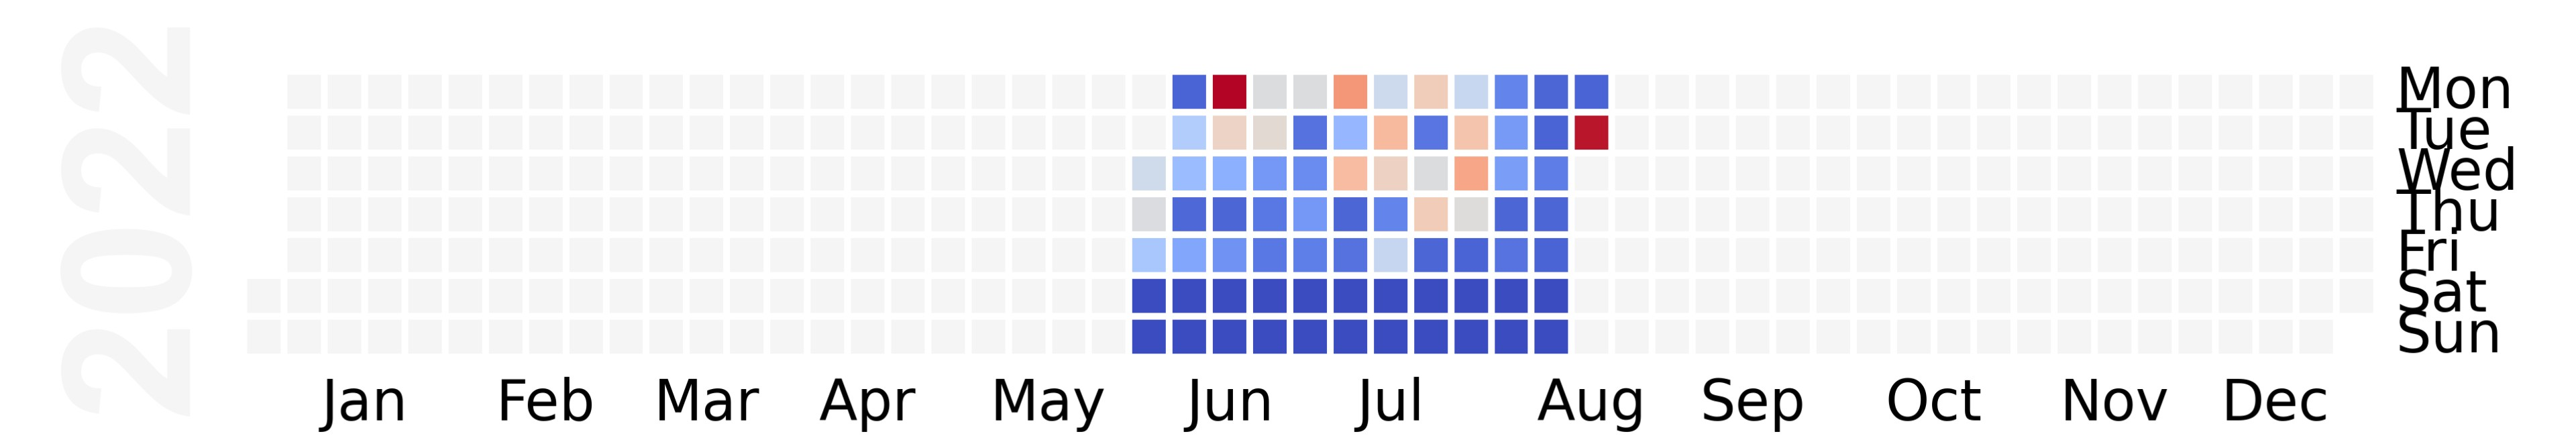
\includegraphics[width=\textwidth]{images/heatmaps/devicetype_Utility_workday_cal.png}
	\caption{Heat map of the sum of all utility sensors during usual office hours (measured during \glspl{workday}).}
	\label{fig:util_hm}
\end{figure}

\subsubsection{\acrfull{rpmt}}\label{subsec:RPMT}
To allow an even more interactive approach to data exploration, the Grafana service as described in the section \ref{subsec:software} allows creation of interactive dashboards. As an example application, in this work a sample dashboard that aims to be used as a motivational tool can be examined. A full screenshot of the dashboard can be seen in figure \ref{fig:dashboard}.\\
Besides showing overview data, Grafana can be used to send notifications if certain thresholds are crossed, for example by using telegram or discord bots. Address to access the Grafana service is shown in table \ref{tab:access} located of section \ref{subsec:hardware}.
\begin{figure}[h]
	\centering	
	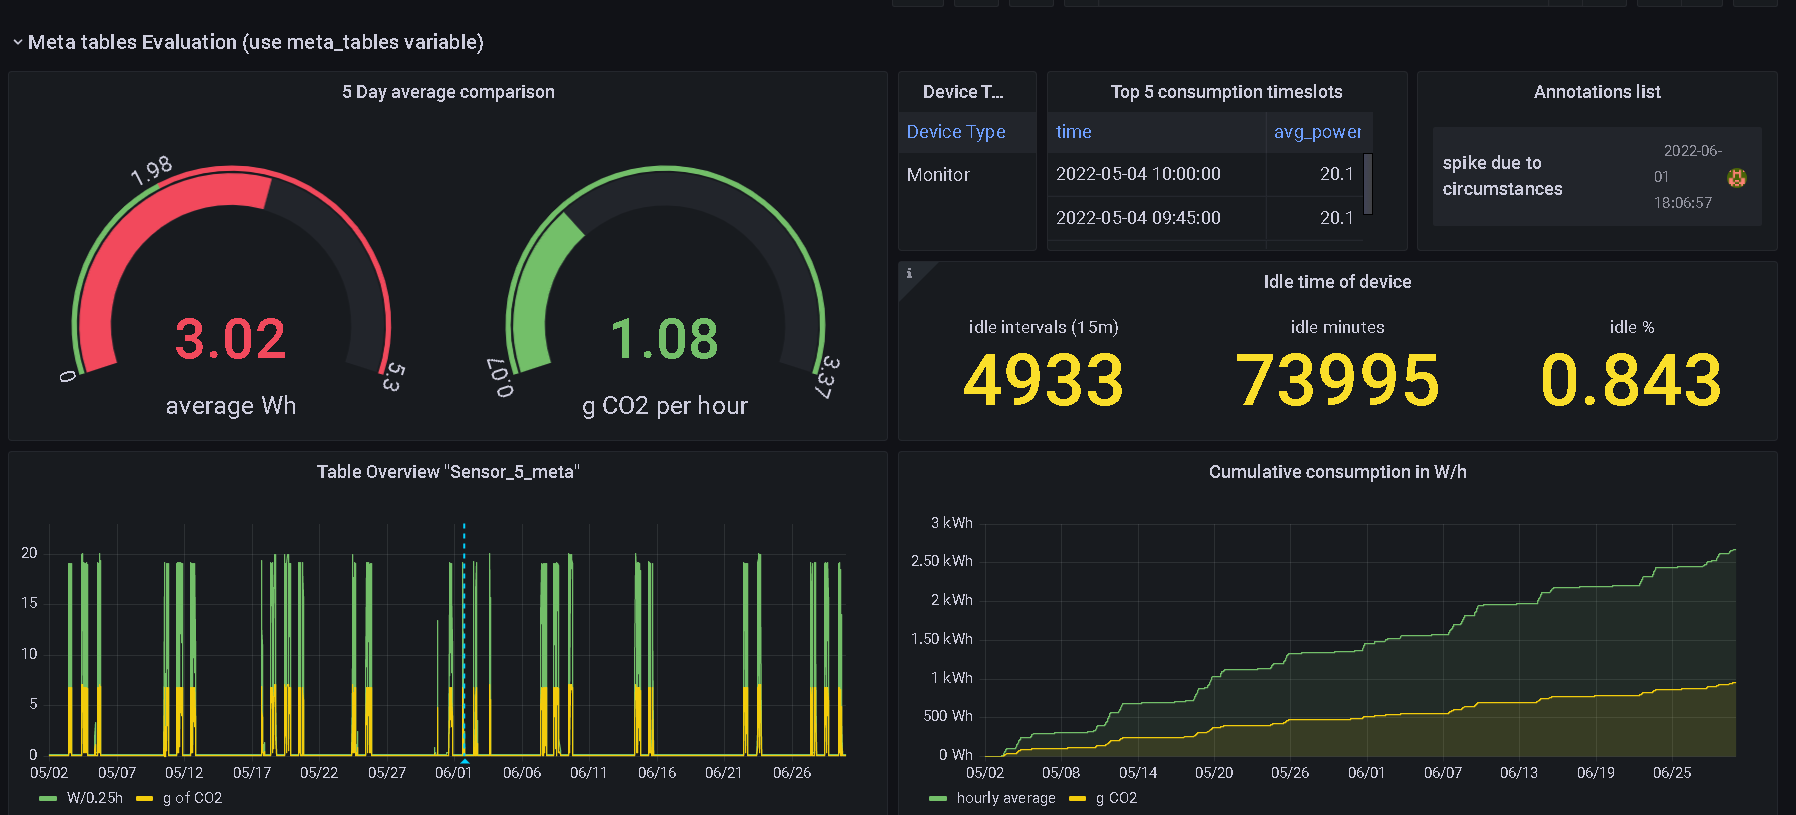
\includegraphics[width=\textwidth]{images/RPMT.png}
	\caption{Screenshot of the \acrshort{rpmt} dashboard. From top left to bottom right there are panels showing 5 day comparisons to similar devices, the device type, an overview of annotations, the overview of elapsed idle time of the device. the power consumption as a time series, and the cumulative time series with the respective estimated CO$_2$ footprint.}
	\label{fig:dashboard}
\end{figure}
\chapter{Discussion}\label{chap:discussion}
In this work the three specific goals stated in the introduction are recalled as:
\begin{itemize}
	\item[1.] Generation of a robust and reliable energy consumption data set.
	\item[2.] Estimating the direct impact of consumed electricity on CO$_2$ footprint.
	\item[3.] Use well defined \acrfullpl{kpi} to identify optimization potential in energy consumption.
\end{itemize}
To accomplish the first goal, in this word a methodology to create a realistic live data set of an actual office environment including hardware, software and performance indicators was defined. The goal was achieved by uniformly distribute sensing hardware into a live office environment. By an automated request and pooling program, requested data was accumulated with sufficiently high density in order to increase signal to noise ratio by averaging over fixed intervals. While basic consumption data was collected with faults, see section \ref{sec:datadisscussion}, the order of magnitude can be very accurately determined, and broadly match expected values from the literature.\\
By evaluating modern CO$_2$ estimation protocols, the risk of over fitting CO$_2$ figures through recent, but misleading values was identified, and a conservative estimation was given. By finding a better data source, like increased mandatory reporting of CO$_2$ contributions of all suppliers to the experiments devices, the average estimation should be supplanted by more recent and dynamic methods.\\
The indications in the data using specified \acrshortpl{kpi} was defined in section \ref{sec:metrics}. The evaluation of the idle time metric has shown valuable specific insights in PC and Monitor consumption, while showing only mixed applicability for device agnostic measurements. The modification of parameters according to device specifications is needed to increase reliable indication on energy usage by all kinds of devices. Meanwhile the introduction of \acrfull{wwcr} has shown great promise in differentiating consumers of similar total energy consumption into a ranking of little to great possible potential in energy conservation. While producing multiple positive results, different approaches can be considered to improve the quality of data generation and validation. The individual limitations of the experiment that became obvious during the hardware setup process were:

\paragraph{Controlled environment}is, while working against the idea of creating realistic values, a well defined environment where parameters can be changed if necessary have many benefits. From missing data due to lack of adherence to the usage of sensors, to the fluctuating quality in network capacity, up to the unavailability of certain possibilities, like access to the service behind a firewall. Components that are permanently out of reach for any type of experiment greatly hinder possibilities and have to be accounted for in advance.

\paragraph{Blinding experiments}of this kind will likely increase the veracity of the data. During experimental process and measurement, multiple office workers showed aversion to the prospect of being monitored. While missuses and repercussions can be avoided using privatization and pseudonymization techniques, the knowledge and physical reminder in form of a visible sensor is most likely influencing staff behavior. While this fact could be useful during interventions, a neutral data gathering will be influenced by this.

\paragraph{Counter measurements}using laboratory equipment might be a useful tool to recognize and minimize faulty live data. As the experimenter has no (permanent) immediate connection or access to the devices, it is quite difficult to recognize unrealistic values without further information on the device. For example in the case of this measurement the ratios of consumption due to computation and monitoring match with the estimated ratios found in the related works in section \ref{chap:relatedworks}, however due to the advancements in computing power and flat screen monitoring, it is unclear if this ratio should still hold.

\paragraph{Improved real time CO2 footprint estimation}would be a great asset when the goal is to more accurately react to specific times where energy conservation should be prioritized, as when renewable energies are more readily available during seasons. While there are different API provider giving accurate daily information to renewable energy generation \cite{co2_footprint_api} in a respective region, due to the interconnected grid system it is fundamentally impossible to determine which energy you are using currently. This has to be determined by retroactively reevaluating energy balance and trade between countries(refer to section \ref{sec:co2works} for specifics) and can only be estimated in advance. Another possibility would be a bypass of the grid by using locally generated electricity. As this kind of power would most likely be renewable, the value of this feature in power conservation would still need to be determined

\pagebreak
\paragraph{Incorporating independent measurements}ranging from accurate count of human traffic, self reliant ways to determine efficiency and value of work per energy consumed, or complementing electricity data, like electric bills could improve overall veracity of the key indicators that are at the core of this experiment

\section{Data Discussion}\label{sec:datadisscussion}
During data collection separate evaluations seemed to result in contradicting data. As seen in the visualization of user 7 in figure \ref{fig:user_comparison} and his respective result table, an obvious sensor bias compiled to a significant error. Mixed with the expected measurement noise mainly due to voltage fluctuations, refer to section \ref{sec:vflux}, and a completely unused workplace, the negative consumption summed to a significant reduction in power consumption overall. Utilizing more controlled environments, it needs to be evaluated if simply ignoring a biased sensor, by cutting negative values, if a production of power by the device is categorically impossible, or if adding similar noise to the signal reaches a more accurate result to actual consumption values. Overall consumption and ratios in processing vs. visualizations stayed within the expected range found in the literature. The evaluation using the proposed \gls{kpi} \acrfull{wwcr} gave some insight to differentiate devices and users with possible bigger efficiency gains by experiencing higher off work consumption. To find applicable intervention methods the metric should be evaluated further in future experiments. Using a simple definition of device Idle Time across device types did only prove successful, if the consumption profile of the device matched with the definitions. Especially in the case of multiple devices per sensor, and high energy intensive printer the idle time did not show useful information, as the threshold was passed seldom. The application of CO$_2$ footprint estimations gives a rough estimate on the impact on greenhouse gas emissions, but the efficacy has to be determined using annual report data by the power provider and distributors.

\section{Future Work}
While providing a solid data basis for a real office environment. The data collection is generally only the first step in making an impact in the environment. There are different possibilities to enlarge the scope of this work to improve its usefulness.
\paragraph{Change of context}while office spaces contribute a proper partition of total energy consumption. The service sector only contributes 25\% of overall electricity demand. This evaluates to the third most sector behind industrial 43\% and residential 26\% \cite{enerdata}. To get a chance of meeting environmental sustainability goals as described in section \ref{sec:sustainability}, all other sectors above need at least as much research to tackle the energy conservation goals.
\paragraph{Widen the scope}of office context measurements, and develop concrete aids and methodologies to influence consumption behavior wherever possible. This includes on the one hand a diversification of different kinds of office spaces in different cities and environments. On the other hand, other aspects of IT, service and communications like data centers, AI research and communication infrastructure need to be included to complete the picture of electricity consumption in the office world.
\paragraph{Adapt the current measurement model} to facilitate other kinds of research. A valuable contribution could be a thorough labeling of the data set to enable the use of AI models to be trained on real consumption data, with the aim to facilitate for example narrow artificial intelligence to find solutions to energy optimization problems.
\paragraph{Find a way to privatize}energy consumption measurements. Modern tech companies frequently find ways to encourage individuals to gather data for a specific tech service to use. The examples range from traffic data using phone location to health data in order to receive an insurance bonus. By providing a service to the public, like a tool to enable smart grid exchange between citizens using localized renewable energy generators, when consumption data is freely given, the gathering of data could become a secondary task if a valuable incentive can be given to prospective users. 
\printglossary[type=\acronymtype]

\printglossary

% -- Appendix (optional)
%\begin{appendices}
%    % !TeX spellcheck = en_US
% !TeX encoding = UTF-8
\chapter{Code}

\chapter{Math}

\chapter{Dataset}
%\end{appendices}
\newpage


%%%%%%%%%%%%%%%%%%%%%%%%%%%%%%%%%%%%%%%%%%%%%%%%%%%%%%%%%%%%%%%%%%%%%%%%%%%%%%%%%%%%%%%%%
\backmatter

% -- Bibliography
\printbibliography

% -- Eidesstattliche Erklärung (= Affadavit)
% !TeX spellcheck = de_DE
% !TeX encoding = UTF-8
\chapter{Eidesstattliche Erklärung}

	Hiermit versichere ich, dass ich diese \thesisType{} selbstständig und ohne Benutzung anderer als der angegebenen Quellen und Hilfsmittel angefertigt habe und alle Ausführungen, die wörtlich oder sinngemäß übernommen wurden, als solche gekennzeichnet sind, sowie, dass ich die \thesisType{} in gleicher oder ähnlicher Form noch keiner anderen Prüfungsbehörde vorgelegt habe.

	\vspace{3cm}

	Passau, \thedate

	\vspace{2cm}

	\parbox{8cm}{
		\hrule \strut \theauthor
	}



\end{document}